\chapter{双矩阵博弈中均衡的几何结构}  \label{c9} %中均衡的几何结构

本章讨论两人策略型博弈中均衡的几何结构，并展示如何利用定性的“最优反应示意图”快速识别均衡。这些示意图（例如图\ref{fig:9.4}）将两个混合策略单纯形划分为带有标签的“最优反应区域”，并对每个单纯形的外部进行适当标记，从而使每一个均衡对应于一个“完全标记”的点对 $(x, y)$。这种方法的优势在于，它可以方便地研究$3\times 3$博弈。相比之下，$2\times 2$博弈的结构较为有限，其最优反应线的交点（如图 \ref{fig:6.8}所示）所呈现的情形要简单得多，而$3\times 3$博弈则具有更加丰富多样的结构。


最优反应示意图由Shapley (1974)引入，用来说明Lemke and Howson (1964) 提出的算法（称为莱姆基–豪森算法）。这个算法能够找出双矩阵博弈的一个均衡。该算法也表明，每个非退化双矩阵博弈的均衡个数都是奇数。本章的第\ref{sec9.2}节将介绍最优反应区域，并在第\ref{sec9.3}节阐述莱姆基–豪森算法的原理。这两节内容是每位博弈论学者都应掌握的基础知识，即便对均衡计算兴趣不大的读者也建议阅读这些内容。


本章其余部分将基于这种几何方法，更加详细地介绍两人博弈中均衡的计算。在式\eqref{eq:9.1}所示的 \(3 \times  2\) 双矩阵博弈中，参与人I 的混合策略单纯形 \(X\) 是一个三角形，而参与人 II 的混合策略单纯形 \(Y\) 是一条线段，这类博弈通常应用上包络法（见第\ref{sec6.7}节）。第\ref{sec9.4}节论述 \(3 \times  3\) 博弈的最优反应示意图，该图是细分的三角形。第\ref{sec9.5}节论述博弈的策略等价性。该等价性不改变最优反应及示意图，在实际分析中十分有用。


虽然在低维情况下，将 \(X\) 和 \(Y\) 划分为最优反应区域便于图形化展示，但在一般维度下，如第\ref{sec9.6}节所述，将对方参与人的效用引入为一个额外的变量更为合适。由此得到的“最优反应”多面体刻画了一般维度下期望收益的上包络。一个在数学上更为简洁且等价的对象是“最优反应有界多面体”，它构成了莱姆基–豪森算法的代数实现（即“互补换基法”）的基础，相关内容将在第\ref{sec9.7}节中介绍。第\ref{sec9.8}节进一步说明了如何将互补换基法扩展到退化博弈，从而给出一个不依赖布劳威尔不动点定理的两人博弈均衡存在性的替代证明。


\section{预备知识和学习目标}  \label{sec9.1}

本章是第\ref{c6} 章的延续，所需预备知识包括上包络法（又称“门柱法”）和退化博弈。读者还需回顾与几何相关的基本概念。例如，单纯形的概念已在第 \ref{sec-7.3} 节中介绍，但本章仅涉及如图 \ref{fig:6.5} 所示的混合策略单纯形。此外，无向图的相关概念已在第\ref{chap:7} 章的背景材料部分进行了介绍。

学习本章后，你应该能够:
\begin{itemize}
\item 为每个参与人最多有三种策略的双矩阵博弈绘制最优反应示意图；

\item 借助这些示意图中使用的标签来识别博弈的均衡，并解释标签与最优反应条件之间的联系；

\item 使用示意图展示莱姆基 - 豪森算法计算一个均衡的过程；

\item 解释两人博弈和三人博弈的策略等价性；


\item 理解最优反应多面体、期望收益的上包络和最优反应区域之间的联系；

\item 能够根据互补换基规则对小型字典进行换基操作。
\end{itemize}



\section{最优反应区域的标记法}   \label{sec9.2}


我们的主要示例是一个 \(3 \times  2\) 双矩阵博弈 $(A, B)$，其中
\begin{equation}\label{eq:9.1}
A = \begin{pmatrix}
2 & 0 \\
1 & 2 \\
0 & 3
\end{pmatrix}, \quad
B = \begin{pmatrix}
2 & 0 \\
0 & 1 \\
4 & 1
\end{pmatrix}.
\end{equation}
这与图 \ref{fig:6.7} 右侧的博弈非常相似，如图\ref{fig:9.1} 所示。


对于\(m \times  n\) 双矩阵博弈，我们依次对两个参与人的纯策略进行编号，
\begin{equation}   \label{eq:9.2}
\begin{aligned}
\text{参与人 I 的纯策略（行）} & : 1, \ldots, m， \\
\text{参与人 II 的纯策略（列）} & : m+1, \ldots, m+n .
\end{aligned}
\end{equation}

\begin{figure}[htbp]
  \centering
  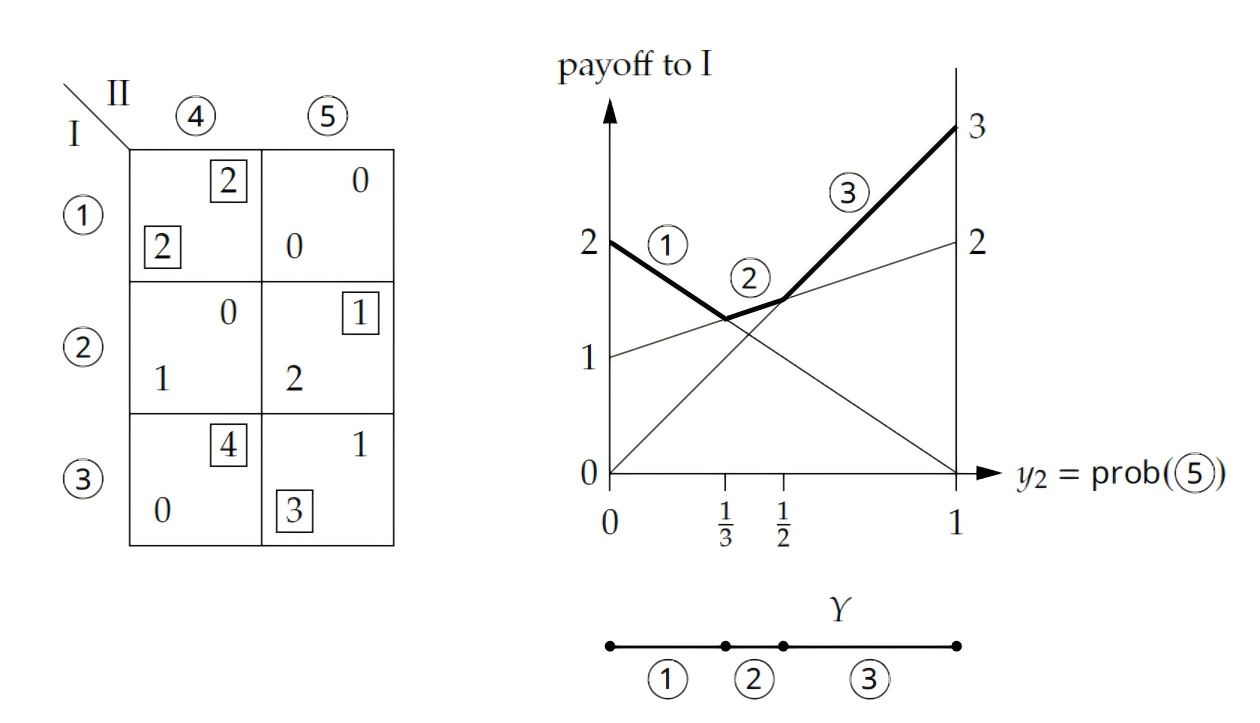
\includegraphics[width=\textwidth]{images/ch09-fig01.png}
  \caption{%
  左图：式~\eqref{eq:9.1} 中的博弈，其中纯策略编号规则如式~\eqref{eq:9.2} 所示。\\  
  右图：对于参与人~II 的混合策略 $y \in Y$，参与人~I 的期望收益上包络。
  混合策略集 $Y$（右下角）被细分为最优反应区域，这些区域用参与人~I 的纯最优反应进行标记。}
  \label{fig:9.1}
\end{figure}



在绘图中，我们通常将它们表示为带圆圈的数字，这里参与人I是$\circled{1}, \circled{2}, \circled{3}$，参与人II是$\circled{4}, \circled{5}$。在本书中，我们通常省略圆圈。


两个参与人的混合策略集 \(X\) 和 \(Y\) 由式 \ref{eq:6.6} 给出。根据式~\eqref{eq:9.2}，我们按照如下规则将它们细分为对方参与人的最优反应区域:
\begin{equation}\label{eq:9.3}
\begin{aligned}
Y(i)
&= \{\, y \in Y \mid i \text{ 是 } y \text{ 的一个最优反应} \},
&& (1 \le i \le m), \\
X(j)
&= \{\, x \in X \mid j \text{ 是 } x \text{ 的一个最优反应} \},
&& (m+1 \le j \le m+n).
\end{aligned}
\end{equation}

由于一个混合策略可能有多个纯最优反应，所以最优反应区域并非不能相交，但这种相交情况通常只发生在最优反应区域的“边界”上。每个混合策略至少有一个最优反应，因此最优反应区域的并集就是相应的混合策略集。在图\ref{fig:9.1}中，\(Y\) 的细分可以从上包络图中看出:
\[
\begin{aligned}
Y(1) &= \left\{ (y_1,y_2) \in Y \;\middle|\; 0 \le y_2 \le \tfrac{1}{3} \right\}, \\
Y(2) &= \left\{ (y_1,y_2) \in Y \;\middle|\; \tfrac{1}{3} \le y_2 \le \tfrac{1}{2} \right\}, \\
Y(3) &= \left\{ (y_1,y_2) \in Y \;\middle|\; \tfrac{1}{2} \le y_2 \le 1 \right\}.
\end{aligned}
\]


图\ref{fig:9.2}展示了将 \(X\) 细分为最优反应区域的情况。策略单纯形 \(X\) 是一个以单位向量 \({e}_{1},{e}_{2}\) 和 \({e}_{3}\) 为顶点的三角形，这些顶点是参与人I的纯策略。如图\ref{fig:9.2}的透视图所示，在每个顶点上竖起一个“球门柱”。在左上图中，这些柱子的高度分别标记为2、0和4，它们表示参与人II选择其左列$\circled{4}$时获得的效用。由此产生的期望收益定义了一个位于三角形上方且穿过这些高度标记的平面，该平面将参与人II选择此列的期望收益定义为 \(x = \left( {{x}_{1},{x}_{2},{x}_{3}}\right)\) 的函数。因为期望收益只是相应“高度”的凸组合，而这些“高度”位于下方三角形 \(X\) 中 \(x\) 点的正上方。类似地，右上图展示了参与人II右列$\circled{5}$时，每个球门柱对应的期望收益0、1和1，它们同样张成了一个期望收益平面。左下图展示了期望收益的上包络，即上述两个期望收益平面的逐点最大值。

\begin{figure}[htbp]
  \centering
  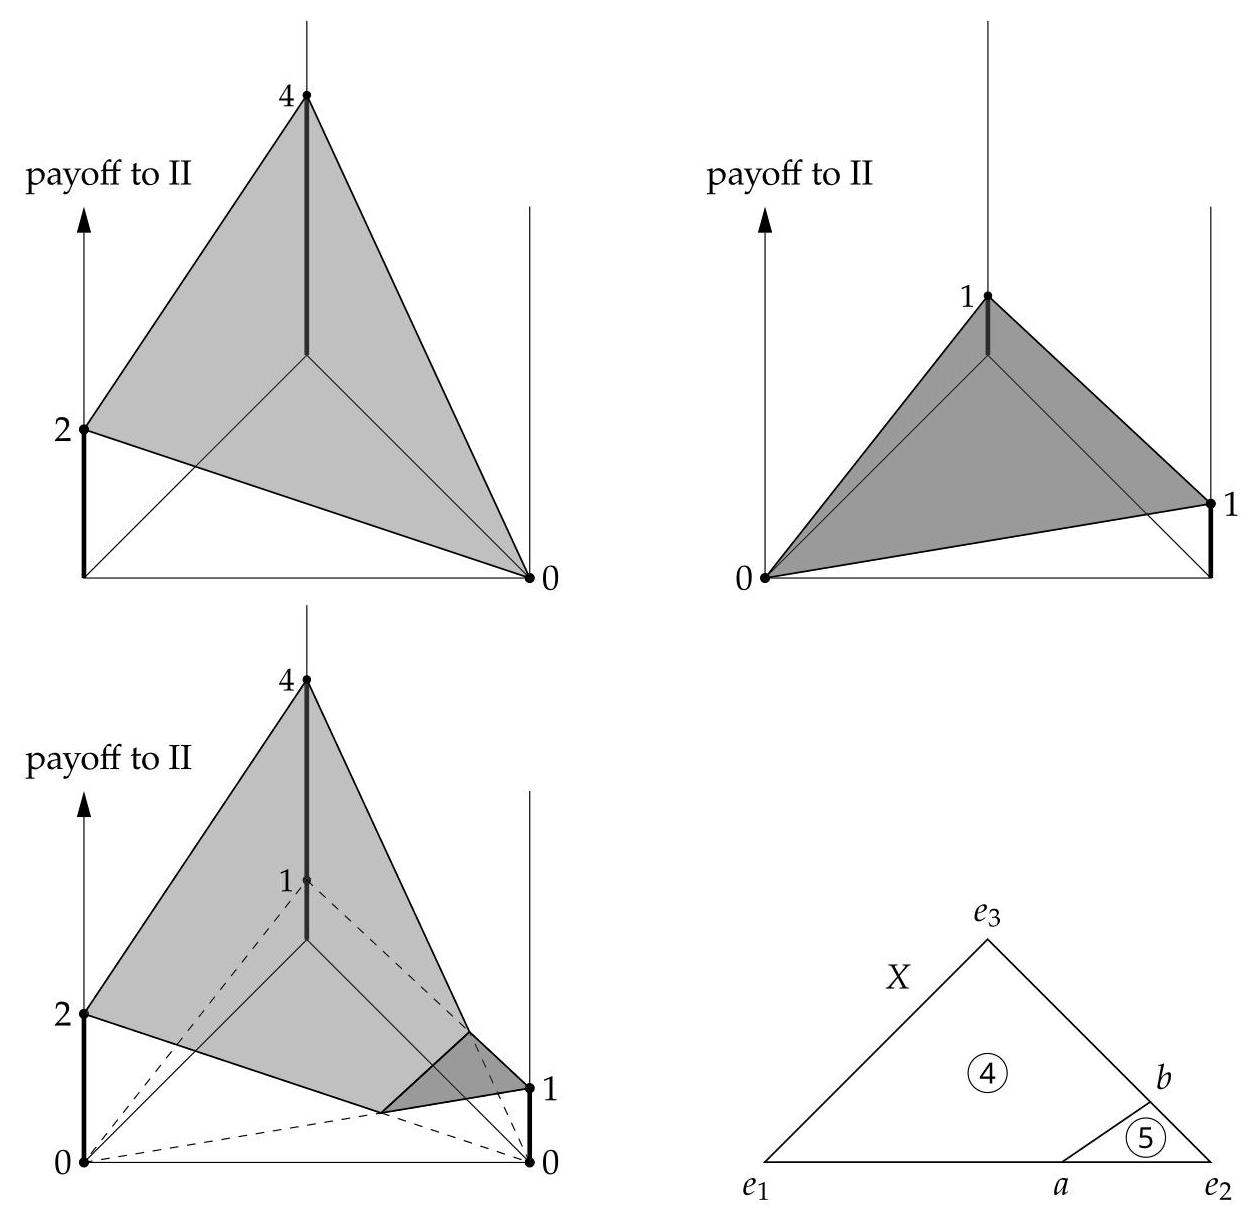
\includegraphics[width=0.9\textwidth]{images/ch09-fig02.jpg}
 \caption{ 对于图\ref{fig:9.1}中的 \(3\times 2\) 博弈，参与人 II 的期望收益是参与人 I 混合策略的函数。左上图：参与人 II 选择左列\protect\circled{4} 的期望收益平面，其在参与人I选择纯策略 $e_1, e_2, e_3$ 时的效用分别为 2，0，4。 右上图：参与人 II 选择右列 \protect\circled{5} 的期望收益平面，其在参与人I选择纯策略 $e_1, e_2, e_3$ 时的效用分别为 0，1，1。左下图：期望收益的上包络（逐点最大值）。右下图：将 $X$ 细分为最优反应区域 $X(4)$ 和 $X(5)$ 的结果。  }
  \label{fig:9.2}
\end{figure}

最后，图\ref{fig:9.2}的右下图展示了期望收益上包络图在 \(X\) 上的“投影”。通过忽略垂直坐标，将 \(X\) 细分为最优反应区域 \(X\left( 4\right)\) 和 \(X\left( 5\right)\)。对于参与人I的混合策略 \(\left( {{x}_{1},{x}_{2},{x}_{3}}\right)\)，参与人II选择左列和右列的期望收益分别为 \(2{x}_{1} + 4{x}_{3}\) 和 \({x}_{2} + {x}_{3}\)。因此，
\[
2{x}_{1} + 4{x}_{3} = {x}_{2} + {x}_{3},
\]
等价地
\begin{equation}\label{eq:9.4}
2 x_1 + 3 x_3 = x_2,
\end{equation}
表示两列的期望收益相等。它在三角形中对应一条同时属于 \(X\left( 4\right)\) 和 \(X\left( 5\right)\)的线段。线段的端点 \(a\) 和 \(b\) （图中已标出）分别由方程 \eqref{eq:9.4} 在 \({x}_{3} = 0\) 时得到 \(a = \left( {\frac{1}{3},\frac{2}{3},0}\right)\)，在 \({x}_{1} = 0\)时得到 \(b = \left( {0,\frac{3}{4},\frac{1}{4}}\right)\)。对于 \(a\) 和 \(b\) 的任意凸组合，该方程也成立，且这些凸组合正好是该线段本身。


在图 \ref{fig:9.1} 和图\ref{fig:9.2}中，式\eqref{eq:9.3}中的最优反应区域 \(Y(i)\) 和 \(X(j)\) 分别用参与人 I 的纯策略 \(i\) 和参与人 II 的纯策略 \(j\) 做了标记。现在，我们通过以下方式，为自身未使用的策略引入第二组标签：
\begin{equation} \label{eq:9.5}
\begin{aligned}
X(i)  &= \left\{  {\left( {{x}_{1},\ldots,{x}_{m}}\right)  \in  X \mid  \;{x}_{i} = 0}\right\},
&& (1 \le i \le m), \\
Y(j) & = \left\{  {\left( {{y}_{1},\ldots,{y}_{n}}\right)  \in  Y \mid  {y}_{j - m} = 0}\right\},
&& (m+1 \le j \le m+n).
\end{aligned}
\end{equation}
这里考虑 \({y}_{j - m}\) 是因为 \(j\) 表示参与人 II 在 \(\{ m + 1,\ldots,m + n\}\) 中的一个纯策略，而 \(y\) 的分量仍有下标 \(1,\ldots,n\)。类似地，参与人 II 的纯策略（即 \(Y\) 的顶点）是 \({\mathbb{R}}^{n}\) 中的单位向量 \({e}_{1},\ldots,{e}_{n}\)。


\begin{definition} \label{def:9.1}  %定义9.1
考虑一个 $m \times n$ 双矩阵博弈 $(A, B)$，其混合策略集分别为式\eqref{eq:6.6} 中的 $X$ 和 $Y$。设 $k \in \{1, \ldots, m+n\}$ 为参与人 I 或参与人 II 的任意纯策略，$X(k)$ 与 $Y(k)$ 分别按式\eqref{eq:9.3} 和 \eqref{eq:9.5} 定义。若 $x \in X(k)$，则称策略 $x \in X$ 具有{标签} $k$；若 $y \in Y(k)$，则称策略 $y \in Y$ 具有{标签} $k$。若对于每一个 $k \in \{1, \ldots, m+n\}$，其均为 $x$ 或 $y$（或两者共同）的标签，则称策略组合 $(x, y)$ 是{完全标记的 }。由这些标签标记的集合 $X$ 与 $Y$ 定义为该博弈的{最优反应图}。
\end{definition}



图 \ref{fig:9.3} 展示了博弈\eqref{eq:9.1}中由式 \eqref{eq:9.5} 定义的未采用自身策略的标签。例如，\(X\left( 1\right)\) 是由 \(X\) 中满足\({x}_{1} = 0\)的点 \(\left( {{x}_{1},{x}_{2},{x}_{3}}\right)\) 构成的三角形的边，这些点是单位向量 \({e}_{2} = \left( {0,1,0}\right)\) 和 \({e}_{3} = \left( {0,0,1}\right)\) 的所有凸组合。一般来说，对于 \(1 \leq  i \leq  m\)，\(X\left( i\right)\) 是三角形中与单位向量 \({e}_{i}\) 对应的顶点相对的极面。参与人 II 的混合策略集 \(Y\) 是一条线段，其端点为 \({e}_{1} = \left( {1,0}\right)\)（即博弈的左列$\circled{4}$）和 \({e}_{2} = \left( {0,1}\right)\)（即博弈的右列$\circled{5}$）。这个低维单纯形 \(Y\) 的每个“边”或极面 \(Y\left( 4\right)\) 或 \(Y\left( 5\right)\) 就是这些端点之一，其中 \({e}_{1}\) 的标签为 5，因为参与人 II 的第二个策略 5 被采用的概率为零（并且这是 \(Y\) 中具有该性质的唯一元素），而另一个端点 \({e}_{2}\) 的标签为 4，因为参与人 II 的第一个策略 4 被采用的概率为零。

\begin{figure}[htbp]
  \centering
  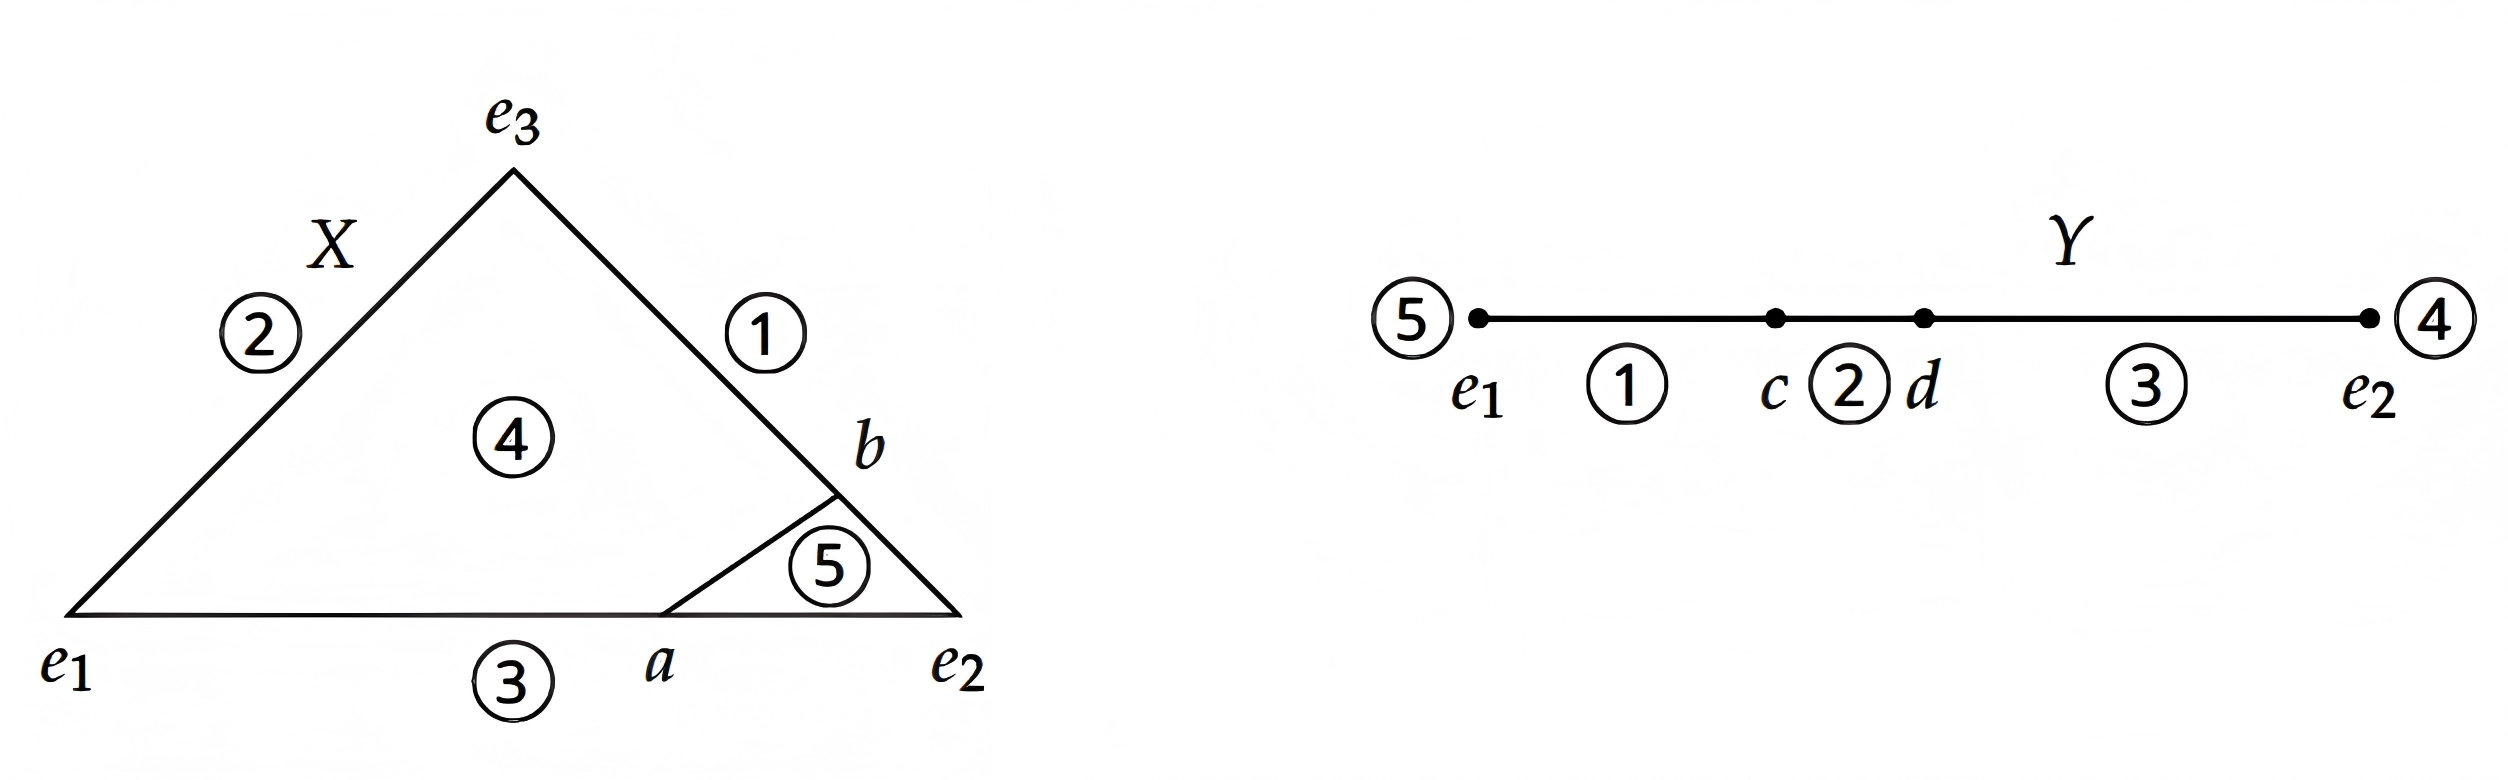
\includegraphics[width=0.9\textwidth]{images/ch09-fig03.png}
 \caption{ 
 图 \ref{fig:9.1}所示博弈的最优反应示意图。图中展示混合策略单纯形 \(X\) 和 \(Y\)，其中最优反应区域以对方参与人的纯策略标记，而边界则以本方未被采用的纯策略标记。
 }
  \label{fig:9.3}
\end{figure}


\begin{figure}[htbp]
\centering
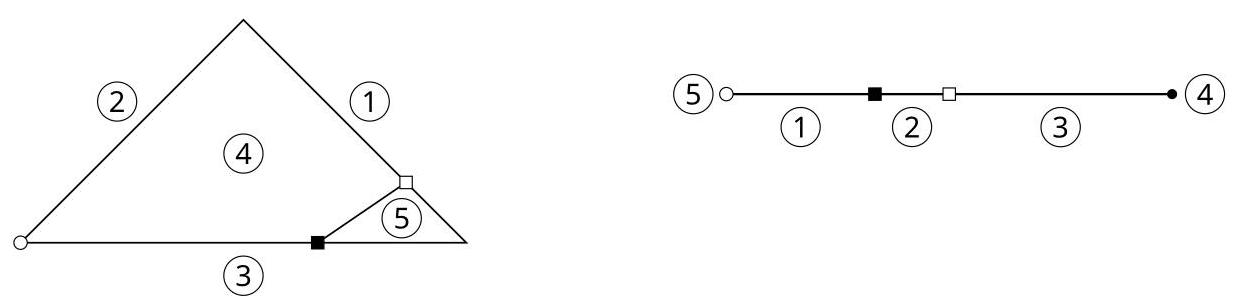
\includegraphics[width=0.9\textwidth]{images/ch09-fig04.jpg}
\caption{与图 9.3 相同，但省略了除标签之外的所有注释，这些标签完全定义了最优反应示意图。完全标记的顶点对均衡用符号表示：白色圆圈表示纯策略均衡 $\left(e_1, e_1\right)$，黑色方块表示 $(a,c)$，白色方块表示 $(b,d)$。}
\label{fig:9.4}
\end{figure}


根据定义 \ref{def:9.1}，任何混合策略 \(x\) 或 \(y\) 可能对应多个标签。将未使用的纯策略也纳入这些标签之中，是为了应用下面这个十分有用的定理。


\begin{theorem}\label{theo:9.2}   %定理 9.2
在定义\ref{def:9.1}的假设下，混合策略组 $(x, y)$ 是 $(A, B)$ 的一个均衡，当且仅当 $(x, y)$ 是完全标记的。
\end{theorem}


\begin{proof}
该定理本质上是最优反应条件（命题\ref{prop:6.1}） 的另一种陈述方式。设 \(\left( {x,y}\right)  \in  X \times  Y\)，设 \(u\) 是参与人 I 针对 \(y\) 的最优反应收益，设 \(v\) 是参与人 II 针对 \(x\) 的最优反应收益，如式\eqref{eq:6.9} 中所定义。假设 $(x, y)$ 是一个均衡，则 \(x\) 是对 \(y\) 的最优反应，如式\eqref{eq:6.11} 所示，并且 \(y\) 是对 \(x\) 的最优反应，如式\eqref{eq:6.12} 所示。这些条件可以写为
\begin{equation}\label{eq:9.6}
\begin{aligned}
x_i &= 0 \;\;\text{或者}\;\; (Ay)_i = u, \quad &(1 \le i \le m),\\
y_j &= 0 \;\;\text{或者}\;\; (x^\top B)_j = v, \quad &(1 \le j \le n),
\end{aligned}
\end{equation}
其中第一个条件表明 \(x\) 有标签 \(i\)）因为 \(x \in  X\left( i\right)\)）或者 \(y\) 有标签 \(i\)（因为 \(i\) 是对 \(y\) 的最优反应，因此 \(y \in  Y\left( i\right)\)），第二个条件表明 \(y\) 有标签 \(m + j\) 或者 \(x\) 有标签 \(m + j\)（因为根据式\eqref{eq:9.2} 中纯策略的编号， \(m + j\) 是对 \(x\) 的最优反应）。换句话说，式\eqref{eq:9.6}表明每个标签 \(i \in  \{ 1,\ldots,m\}\) 或 \(m + j \in  \{ m + 1,\ldots,m + n\}\) 都作为 \(x\) 或 \(y\) 的标签出现，因此 $(x, y)$是完全标记的。


相反，如果 $(x, y)$ 是完全标记的，那么式\eqref{eq:9.6}成立，且 \(x\) 和 \(y\)互为最优反应，因此$(x, y)$是一个均衡。
\end{proof}


另一种快速理解定理\ref{theo:9.2} 的方法是：如果$(x, y)$ 缺失某个标签，那么该标签对应的必然是某个参与人以正概率选择的纯策略（因为它并不像式\eqref{eq:9.5}中的情形那样是一个未采用的纯策略），并且它也不是一个最优反应。这恰恰违反了最优反应条件的要求，并且不满足式\eqref{eq:9.6}。两个参与人的纯策略按照式\eqref{eq:9.2}分别编号，这样这些策略就可以作为 \(x\) 或 \(y\) 的标签出现，并且也助于区分式\eqref{eq:9.6}中的两组条件。


如图\ref{fig:9.3} 所示，\(X\) 中只有点\({e}_{1},{e}_{2},{e}_{3},a,b\) 有三个标签（这是 \(X\) 中一个点的最大标签数），而集合 \(Y\) 中只有点 \({e}_{1},{e}_{2},c,d\) 有两个标签（这是 \(Y\) 中一个点的最大标签数）。一个均衡 $(x, y)$ 需要参与人纯策略的所有五个标签，因此可以迅速识别出该博弈的均衡。具体为：

\begin{itemize}
\item 纯策略均衡 \(\left( {{e}_{1},{e}_{2}}\right)\)，在 \(X\) 中有标签 2、3、4（这意味着 2 和 3 未被采用，4 是最优反应），在 \(Y\) 中有标签 5和1（这意味着 5 未被采用，1 是最优反应）。这个均衡在图 \ref{fig:9.4}中用白色圆圈标记。

\item 混合策略纳什均衡 $(a, c)$，对于 \(X\) 中的 \(a = \left( {\frac{1}{3},\frac{2}{3},0}\right)\) 有标签 3、4、5（这意味着 3 未被采用，4 和 5 是最优反应），对于 \(Y\) 中的 \(c = \left( {\frac{2}{3},\frac{1}{3}}\right)\) 有标签 1和2（这意味着 1 和 2 都是最优反应）。这在图\ref{fig:9.4} 中用黑色方块标记。

\item 混合策略纳什均衡 $(b, d)$，对于 \(X\) 中的 \(b = \left( {0,\frac{3}{4},\frac{1}{4}}\right)\) 有标签 1、4、5（这意味着 1 未被采用，4 和 5 是最优反应），对于 \(Y\) 中的 \({\color{red}d} = \left( {\frac{1}{2},\frac{1}{2}}\right)\) 有标签 2和3（这意味着 2 和 3 都是最优反应）。这在图 \ref{fig:9.4} 中用白色方块标记。  % 坐标将c更正为d
\end{itemize}


寻找这些作为完全标记点对的均衡，最快方法是检查集合\(Y\) 中具有两个标签的点，此时补全完整标签集合所需的另外三个标签是唯一的，这些标签可能出现在 $X$ 中的某些点上，也可能不出现。集合  \(Y\) 中的三个点 \({e}_{1},c,d\) 均属于某个均衡，但\({e}_{2}\)不属于均衡。这是由于\({e}_{2}\)有标签 3 和 4，而所需的另外三个标签 1、2、5 没有出现在 \(X\) 中，其判断依据是集合 \(X\left( 2\right)\) 和 \(X\left( 5\right)\) 没有公共点。这种方法足以找到所有的均衡。另一个类似但稍微繁琐的方法是：检查 $X$ 中标签为 1、3、5的点 ${e}_{2}$，此时 $Y$ 中没有点具有其他两个标签 2 和 4；检查$X$ 中标签为 1、2、4的点${e}_{3}$，此时$Y$ 中没有点具有其他两个标签 3 和 5。

博弈的最优反应示意图的优点在于：它是一种定性图示，能够识别纳什均衡，并且相比收益矩阵而言，提供更加丰富的信息。在图\ref{fig:9.4}中，我们仅将标签作为注释保留，不过这些标签仍然编码了所有必要的信息。特别地，\(X\) 是参与人I的策略集，因为其边上的标签是参与人I的纯策略，而内部标签是参与人II的纯最优反应；对于 \(Y\)，情况则相反。 \(X\) 的顶点是单位向量，通过未使用纯策略的标签来识别。例如，\({e}_{1} = \left( {1,0,0}\right)\) 是具有标签2和3的顶点。在 \(Y\) 中，对于参与人II的第一个策略 \({e}_{1} = \left( {1,0}\right)\)，未采用的纯策略标签是 \(5 = m + 2\)，它对应\(Y\)的该端点；而对于 \(Y\) 的第二个端点 \({e}_{2} = \left( {0,1}\right)\)，其标签为 \(4 = m + 1\)。均衡本身则可以通过它们互补的标签集来识别。


\section{莱姆基 - 豪森算法}  \label{sec9.3}


根据定理\ref{theo:9.2}，通过完全标记的点对$(x, y)$可以识别均衡，但尚未证明这样的点对一定存在。图\ref{fig:9.5}是图\ref{fig:9.3}的扩展，它展示了这种存在性的证明方法，而这正是本节要讨论的主题。一般来说，该方法为找到非退化 \(m \times  n\) 双矩阵博弈的一个均衡提供了一种算法，该算法由Lemke and Howson (1964) 提出。在下面的第\ref{sec9.7}节中，我们将给出该算法更具体也更严格的描述，该描述也适用于退化博弈。这为两人博弈中均衡的存在性提供了一个新的、基本的证明方法，并且不需要布劳威尔不动点定理。然而，这个证明与用于证明不动点定理的技术有一些相似之处，特别是在斯佩纳引理的证明中使用的“奇偶性论证”。



混合策略集 \(X\) 是 \({\mathbb{R}}^{m}\) 的一个子集，\(Y\) 是 \({\mathbb{R}}^{n}\) 的一个子集。 \(X\) 和 \(Y\) 分别不包含 \({\mathbb{R}}^{m}\) 或 \({\mathbb{R}}^{n}\) 的原点$\mathbf{0}$。我们现在将$\mathbf{0}$添加到 \(X\) 中，并通过线段将其连接到 \(X\) 的每个顶点 \({e}_{1},\ldots,{e}_{m}\)，并将 \(X\) 的这个扩展记为 \(\widetilde{X}\)。类似地，将$\mathbf{0}$添加到 \(Y\) 中，并将得到的扩展记为 \(\widetilde{Y}\)。图\ref{fig:9.5}展示了例\eqref{eq:9.1}中的 \(\widetilde{X}\) 和 \(\widetilde{Y}\)。


然后，根据式\eqref{eq:9.5}，\(\widetilde{X}\) 中的$\mathbf{0}$具有所有标签 \(1,\ldots,m\)，\(\widetilde{Y}\) 中的$\mathbf{0}$具有所有标签 \(m + 1,\ldots,m + n\)。因此，$(\mathbf{0}, \mathbf{0})$是完全标记的，并称其为 \(\widetilde{X} \times  \widetilde{Y}\) 的人工均衡（artificial equilibrium）。它不代表一个混合策略组。


我们现在将 \(\widetilde{X}\) 和 \(\widetilde{Y}\) 视为图，就像图 \ref{fig:9.5} 中所绘制的那样。图 \(\widetilde{X}\) 的节点是具有 \(m\) 个标签的点；如果两个节点共享 \(m - 1\) 个标签，则它们之间通过一条边相连，这些共同的标签就是该边的标签。例如，节点$\mathbf{0}$（标签为 1、2、3）和 \({e}_{2}\)（标签为 1、3、5）之间由具有标签 1 和 3 的边相连。图 \(\widetilde{Y}\) 的节点是具有 \(n\) 个标签的点，如果两个节点有 \(n - 1\) 个共同标签（在图 \ref{fig:9.5} 中的边只有一个标签，因为 \(n - 1 = 1\)），则通过一条边相连，这些标签就是该边的标签。


\begin{figure}[ht]
\centering
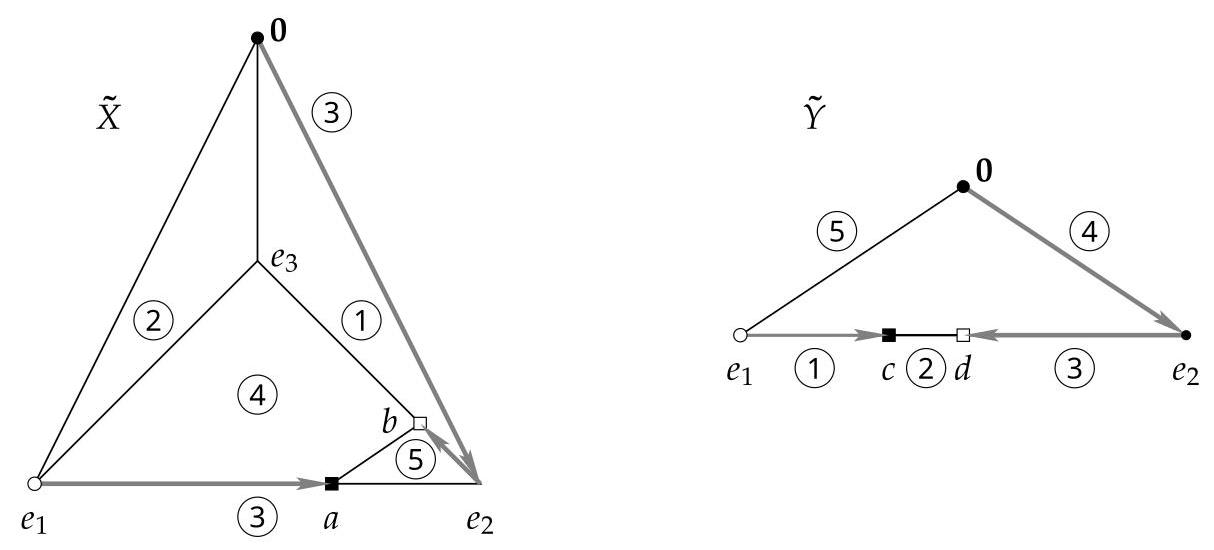
\includegraphics[width=0.8\textwidth]{images/ch09-fig05.jpg}
\caption{图 \ref{fig:9.3}中标记的混合策略集 $X$ 和 $Y$，每个都通过一个所有分量都为零的额外点 $\mathbf{0}$ 进行扩展，使得 $(\mathbf{0},\mathbf{0})$ 是一个完全标记的“人工均衡”。灰色箭头表示缺失标签 2 的两条莱姆基–豪森路径。这些路径的端点是人工均衡和博弈的均衡，因此均衡的数量是奇数。}
\label{fig:9.5}
\end{figure}


接下来，我们在 \(\{ 1,\ldots,m + n\}\) 中选择一个允许缺失的标签，并在后续过程中保持该标签固定不变。我们考虑所有满足如下条件的点对 \((x,y)\in \widetilde{X} \times  \widetilde{Y}\)：它们包含除该允许缺失标签之外的所有标签；并将这样的点对 $(x, y)$ 称为几乎完全标记的。几乎完全标记的点对 $(x, y)$ 属于两种类型的集合。第一类形式为 \(\{ x\}  \times  E\)，其中 \(x\) 是 \(\widetilde{X}\) 的一个节点， \(E\) 是 \(\widetilde{Y}\) 的一条边。对于\(x\)，具有 \(m\) 个标签；对于\(y \in  E\)，具有 \(n - 1\) 个标签，除了边\(E\) 的两个端点外，因为端点有 \(n\) 个标签。第二类形式为\(E \times  \{ y\}\)，其中 \(E\) 是 \(\widetilde{X}\) 的一条边，\(y\)是\(\widetilde{Y}\) 中的一个节点。对于\(x \in  E\)，具有 \(m - 1\) 个标签，除了边\(E\) 的两个端点外，因为端点有 \(m\) 个标签；对于\(y\)，具有 \(n\) 个标签。（严格来说，这些集合是两个图 \(\widetilde{X}\) 和 \(\widetilde{Y}\) 的乘积图的边。）



在图\ref{fig:9.5}中，选择的缺失标签为2。根据定义，任何完全标记的点对 $(x, y)$ 同时也是几乎完全标记的。它作为几乎完全标记的点对$(x, y)$构成的一条路径的唯一起始点。我们从人工均衡$(\mathbf{0}, \mathbf{0})$开始。由于允许标签2缺失，我们去掉标签2，这意味着在保持 \(y = \mathbf{0}\) 固定不变的情况下，使$x$沿着\(\widetilde{X}\)中连接点$\mathbf{0}$和 \({e}_{2}\) 的唯一边移动（该边在 \(\widetilde{X}\) 中用箭头表示）。在\(\widetilde{X}\) 中该箭头的终点 \(x = {e}_{2}\) 获得了一个新的标签5。因为此时 \(x\) 有三个标签1、3、5，而 \(y = \mathbf{0}\) 有两个标签4、5，即标签2缺失，所以在 \(\widetilde{X}\) 中刚获得的标签5现在是重复标签。因为 \(y\) 不再需要重复标签5，下一步是在 \(\widetilde{Y}\) 中去掉标签5，即沿着只有标签4的边将 \(y\) 从$\mathbf{0}$改变到 \({e}_{2}\)。在 \(\widetilde{Y}\) 中该边的终点 \({e}_{2}\) 有标签4和3，其中标签3在$x$中已被获取。因此，当前的点对 \(\left( {x,y}\right)  = \left( {{e}_{2},{e}_{2}}\right)\) 有重复标签3。相应地，我们现在可以在 \(\widetilde{X}\) 中去掉标签3，即沿着带有标签1和5的边将 \(x\) 移动到点 \(b\)，在那里获取标签4。当前的点对 \(\left( {x,y}\right)  = \left( {b,{e}_{2}}\right)\)，标签4是重复标签。接下来，我们通过沿着\(\widetilde{Y}\) 中具有标签3的边移动\(y\)，去掉标签4，以到达点 \(d\)，此时获取标签2。因为2是预先允许缺失的标签，所以到达的点对 \(\left( {x,y}\right)  = \left( {b,d}\right)\) 是完全标记的。这就是在路径终点处找到的均衡。总之，该路径由 \(\widetilde{X} \times  \widetilde{Y}\) 中的一系列点以及相应的标签集合给出
\begin{equation} \label{eq:9.7}
\begin{array}{cccc}
\hline 
(x, y) & & \text{标签} & \text{去掉的标签} \\
\hline
(\mathbf{0},\mathbf{0}) & \bullet & 123,45 & \widetilde{X} \mbox{中的标签 }2 \\
%\hline
(e_2,\mathbf{0}) & & 135,45 & \widetilde{Y} \mbox{中的标签 } 5 \\
%\hline
(e_2,e_2) & & 135, 43 & \widetilde{X} \mbox{中的标签 } 3\\
%\hline
(b,e_2) & & 145, 43 & \widetilde{Y} \mbox{中的标签 } 4\\
%\hline
(b,d) & \square & 145, 23 & \ \text{（}\widetilde{Y} \mbox{中找到了标签 } 2\text{）} \\
\hline
\end{array}
\end{equation}


因此，从人工均衡$(\mathbf{0},\mathbf{0})$开始，由\(\widetilde{X} \times  \widetilde{Y}\) 中几乎完全标记的节点对构成的序列终止在该博弈的一个实际均衡。一般来说，这就构成了由Lemke 和 Howson (1964) 提出的用于寻找双矩阵博弈均衡的算法。因此，式\eqref{eq:9.7}中的路径也被称为缺失标签为2的莱姆基 - 豪森路径。注意，该路径在 \(\widetilde{X}\) 和 \(\widetilde{Y}\) 之间交替移动：在每一步中，固定$(x, y)$中的一个分量 \(x\) 或 \(y\)，并通过沿着相应图 \(\widetilde{Y}\) 或 \(\widetilde{X}\) 中的一条边来改变另一个分量。


莱姆基 - 豪森路径可以从任何完全标记的点对$(x, y)$开始，而不仅仅是从人工均衡开始。例如，如果从图\ref{fig:9.5}中的$(b, d)$开始，那么（缺失标签2的）路径只是反向遍历路径\eqref{eq:9.7}，然后会回到$(\mathbf{0},\mathbf{0})$。然而，该博弈还有其他均衡，例如由白色圆圈表示的纯策略均衡 \(\left( {{e}_{1},{e}_{1}}\right)\)。从这个均衡开始，缺失标签为2的莱姆基 - 豪森路径也在图\ref{fig:9.5}中显示。该路径只包含两步，最终到达第三个均衡$(a, c)$:
\begin{equation} \label{eq:9.8}
\begin{array}{cccc}
\hline
(x, y) &  & \text{标签} & \text{去掉的标签} \\
\hline
(e_1, e_1) & \circ & 234, 15 & \widetilde{X} \mbox{中的标签 } 2\\
%\hline
(a, e_1) &   & 345, 15 &\widetilde{Y} \mbox{中的标签 } 5 \\
%\hline
(a, c) & \blacksquare & 345, 12 &  \text{（}\widetilde{Y} \mbox{中找到了标签 } 2\text{）} \\
\hline
\end{array}
\end{equation}





因此，对于给定的缺失标签，博弈的均衡加上人工均衡是莱姆基 - 豪森路径的端点。由于每条路径有两个端点，所以它们的总数是偶数，从而博弈的均衡数量是奇数。这是一个奇偶性论证，类似于第\ref{sec-7.4}节中用于斯珀纳引理的论证。


为了对一般的双矩阵博弈进行这种奇偶性论证，我们必须假设该博弈是非退化的（见定义~\ref{def:6.7}），因为退化博弈不一定有奇数个均衡。例如，图~\ref{fig:6.12}中的退化博弈的均衡集合是无限集（借助最优反应示意图可以很好地理解这一点，见练习~\ref{exer:9.2}）。


\begin{lemma}\label{lem:9.3}   % 引理9.3
定义\ref{def:9.1}中的 \(m \times  n\) 双矩阵博弈是非退化的，当且仅当 \(X\) 中没有点的标签超过 \(m\) 个，且 \(Y\) 中没有点的标签超过 \(n\) 个。
\end{lemma}

\begin{proof}
设 \(x = \left( {{x}_{1},\ldots,{x}_{m}}\right)  \in  X\)，考虑集合 \(I = \left\{  {i \mid  {x}_{i} = 0,1 \leq  i \leq  m}\right\}\) 和 \(J = \{ j \mid  j\) 是对 \(x \) 的最优反应, \(m + 1 \leq  j \leq  m + n\}\)，因此 \(I \cup  J\) 是 \(x\) 的标签集合。\(x\) 以正概率采用的纯策略数量是 \(m - \left| I\right|\)，而非退化性要求 \(\left| J\right|  \leq  m - \left| I\right|\)，或者等价地 \(\left| I\right|  + \left| J\right|  \leq  m\)，即 \(x\) 的标签不超过 \(m\) 个。类似地，在非退化博弈中，任何 \(y \in  Y\) 的标签都不超过 \(n\) 个。在退化博弈中，对于某些 \(x\) 或 \(y\)，这一条件不成立。
\end{proof}


对于非退化的 \(m \times  n\) 博弈，图 \(\widetilde{X}\) 和 \(\widetilde{Y}\) 具有以下性质（我们没有给出证明，因为我们将在第\ref{sec9.7}节中给出莱姆基 - 豪森方法的另一种更严格的描述）:


\begin{itemize}
\item \(\widetilde{X}\) 的节点是 \(X\) 中具有 \(m\) 个标签的有限个点，再加上 \(\mathbf{0} \in  {\mathbb{R}}^{m}\)。 \(\widetilde{Y}\) 的节点是 \(Y\) 中具有 \(n\) 个标签的有限个点，再加上 \(\mathbf{0} \in  {\mathbb{R}}^{n}\)。


\item 如果 \(\widetilde{X}\) 的任意两个节点有 \(m - 1\) 个共同的标签，那么这两个节点由一条边相连，且这些共同标签就是该边的标签（作为一个几何对象，这条边是至少具有这些标签的点的集合；作为图 \(\widetilde{X}\) 的一条边，这条边由 \(\widetilde{X}\) 中的一对节点 \(\left\{  {x,{x}^{\prime }}\right\}\)表示）。如果 \(\widetilde{Y}\) 的任意两个节点有 \(n - 1\) 个共同的标签，那么这两个节点由一条边相连，且这些共同标签就是 \(\widetilde{Y}\) 中该边的标签。

\item 对于 \(\widetilde{X}\) 中的任意节点 \(x\) 以及 \(x\) 的一个标签 \(k\)，\(\widetilde{X}\) 中存在唯一一条以 \(x\) 为端点的边，该边包含 \(x\) 的除 \(k\) 之外的所有标签。我们称这条边是通过去掉标签 \(k\) 从 \(x\) 遍历得到的（这条边 \(\left\{  {x,{x}^{\prime }}\right\}\) 的另一个端点 \({x}^{\prime }\) 会获得一个不同于\(k\)的新标签，如图 \ref{fig:9.5} 所示）。同样的情况适用于 \(\widetilde{Y}\) 中的任意节点。
\end{itemize}

设 \(\ell  \in  \{ 1,\ldots,m + n\}\)。利用上述性质，我们将缺失标签 \(\ell\) 的莱姆基 - 豪森图（简称为LH图）定义为 \(\widetilde{X}\) 和 \(\widetilde{Y}\) 的“乘积图”的某个子集。LH 图的节点是 \(\widetilde{X} \times  \widetilde{Y}\) 中几乎完全标记的节点对 $(x, y)$，即 \(\{ 1,\ldots,m + n\}  - \{ \ell \}\) 中的每个标签都作为 \(x\) 或 \(y\) 的标签出现。LH 图中的任意一条边具有如下两种形式之一：\(\left\{  {\left( {x,y}\right),\left( {x,{y}^{\prime }}\right) }\right\}\)，其中 \(\left\{  {y,{y}^{\prime }}\right\}\) 是 \(\widetilde{Y}\)中的一条边；\(\left\{  {\left( {x,y}\right),\left( {{x}^{\prime },y}\right) }\right\}\)，其中 \(\left\{  {x,{x}^{\prime }}\right\}\) 是 \(\widetilde{X}\) 中的一条边。如果 $(x, y)$ 是完全标记的点对，那么它在 LH 图中有唯一一个邻居，该邻居通过去掉标签 \(\ell\) 到达，即沿着不包含标签 \(\ell\) 的那条边移动（如果 \(\ell  \in  \{ 1,\ldots,m\}\)，则沿着 \(\widetilde{X}\) 中的边移动；否则沿着\(\widetilde{Y}\) 中的边移动）。如果$(x, y)$是几乎完全标记且不包含标签 \(\ell\)的点对，那么恰好存在一个重复标签 \(k\)，该标签同时作为 \(x\) 和 \(y\) 的标签出现。LH 图中这样的节点恰好有两个邻居，分别对应于在 \(\widetilde{X}\) 或 \(\widetilde{Y}\) 中去掉重复标签 \(k\) 到达的节点。


在双矩阵博弈中，因为 LH 图中的每个节点 $(x, y)$ 的度为 1 或 2，所以该图是由路径和环组成的集合。路径的端点是度为 1 的节点，从而这些端点的数量必然是偶数。其中一个端点是人工均衡$(\mathbf{0},\mathbf{0})$，而其他每个端点都是该博弈的一个均衡。至此，奇偶性论证完成。我们将其总结为一个定理（其完整证明需要证明上述各项性质）。


\begin{theorem} \label{theo:9.4}  % 定理 9.4
一个非退化的双矩阵博弈有奇数个均衡。
\end{theorem}

\begin{figure}[htbp]
\centering
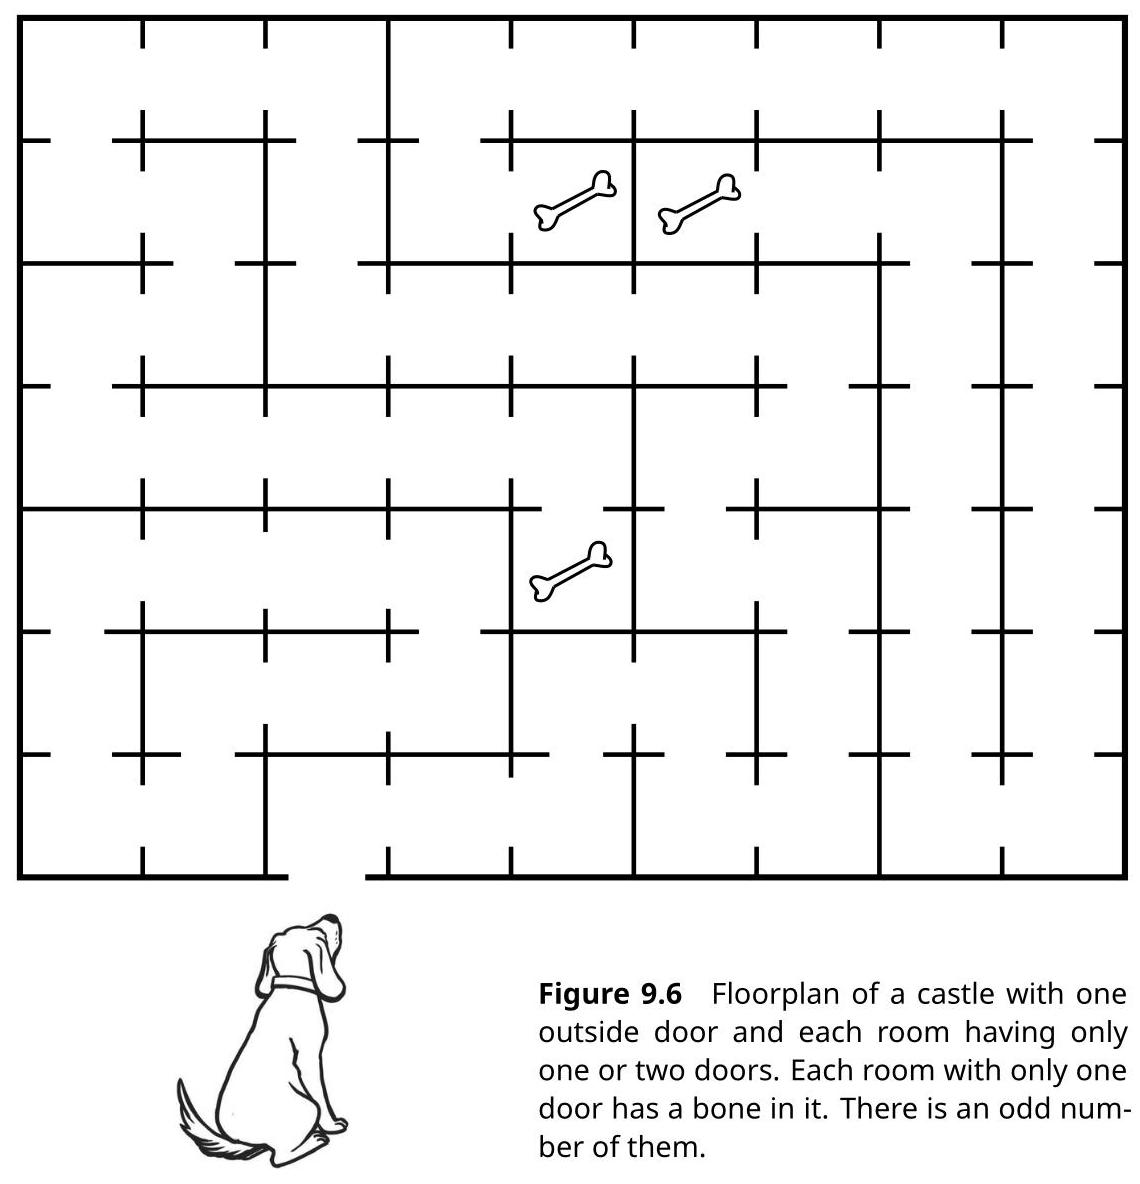
\includegraphics[width=0.8\textwidth]{images/ch09-fig06.jpg}
\caption{这是一座城堡的平面图。每个房间只有一扇或两扇门，只有一扇门通向城堡外面。只有一扇门的每个房间里都放着一根骨头，这类房间的总数是奇数。}
\label{fig:9.6}
\end{figure}



记住这种奇偶性论证的一种方式，是通过一座城堡的故事。这座城堡里的房间构成了一个迷宫（不过，它不是真正的迷宫，因为进入其中后不会走错路），如图\ref{fig:9.6}所示。城堡里的每个房间只有一扇或两扇门。只有一扇门通向城堡外面，其他每扇门都通向另一个房间。每个只有一扇门的房间里都有一根骨头。一只饥饿的狗来到城堡，能够很容易地找到一根骨头，过程如下：狗从外部的门进入城堡，并进入一个房间。如果该房间中有一根骨头，狗就找到了目标；如果该房间有两扇门，则狗从该房间的另一扇门出去，并继续以同样的方式前进。这样，狗穿过了城堡里的一些房间，但不会再次进入同一个房间，因为要再次进入那个房间就需要第三扇门。狗也无法走出城堡，因为只有一扇门通向外面，而那扇门就是它进来的门。因此，由于城堡中的房间数量有限，这一系列房间访问过程必然会在某处终止，而终点只能是一个只有一扇门并且里面有骨头的房间。在这个类比中，城堡里的一个房间是LH图的一个节点，连接两个房间的一扇门是LH图的一条边。城堡外面是人工均衡。每个只有一扇门（且里面有骨头）的房间是一个均衡。此外，根据定理\ref{theo:9.4}，骨头的数量是奇数，因为从一根骨头出发要么通向城堡外面，要么通向另一根骨头。此外，可能存在所有房间都有两扇门的环路，如图\ref{fig:9.6}左下角所示。



\section{最优反应图}   \label{sec9.4}


本节论述最优反应图在 \(3 \times  3\) 博弈中的应用。对于 \(2 \times  2\) 博弈，我们可以在一个表示 \(X \times  Y\) 的正方形中同时绘制所有混合策略对（如图\ref{fig:6.4}和图\ref{fig:6.8}所示），这样均衡就可以被识别为正方形中的一个点。对于 \(3 \times  3\) 博弈，最优反应图则由分别表示\(X\) 和 \(Y\) 的两个三角形构成，于是每个均衡必须用一个单独的符号分别标识其在\(X\) 和 \(Y\) 中对应的均衡策略，如图\ref{fig:9.4}所示的\(3 \times  2\) 博弈\eqref{eq:9.1}的情形。由于\(3 \times  3\) 博弈相较于 \(2 \times  2\) 博弈包含更多可能的情形，因此借助二维图形对其进行分析是非常有用的方法。


\begin{figure}[ht]
\centering
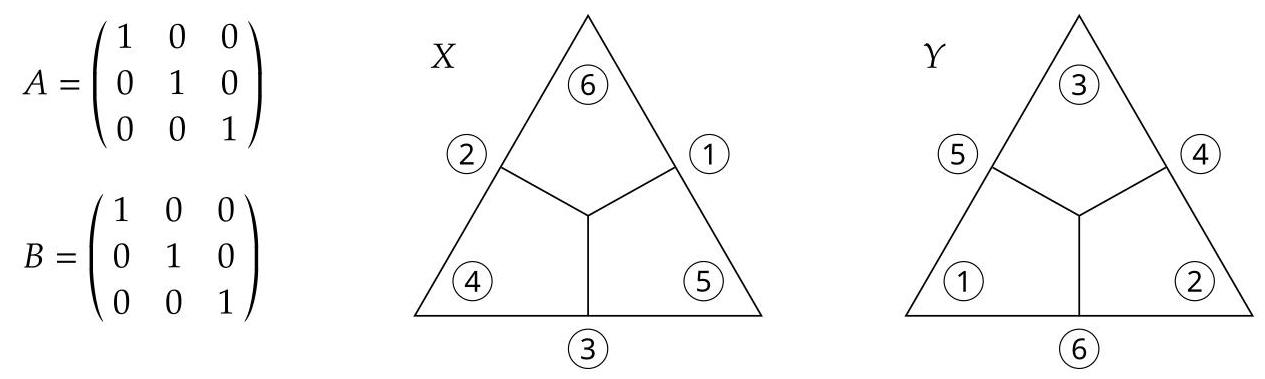
\includegraphics[width=0.9\textwidth]{images/ch09-fig07.jpg}
\caption{$3 \times 3$ 协调博弈 $(A, B)$ 及其最优反应示意图。集合 $X$ 中每个带有三个标签的点与集合 $Y$ 中的对应点共同构成一个均衡，因此该博弈共有七个均衡。}
\label{fig:9.7}
\end{figure}

在一个 \(3 \times  3\) 博弈中，参与人I的策略（即行策略）具有标签1、2、3；参与人II的策略（即列策略）具有标签4、5、6。每个策略集 \(X\) 和 \(Y\) 均为三角形，且最多包含三个最优反应区域。


图\ref{fig:9.7}展示了一个$3\times 3$协调博弈$(A, B)$，其中 \(A\) 和 \(B\) 为单位矩阵。这个协调博弈是对称博弈：如果两个参与人选择相同的行和列，双方均获得收益1；否则，双方收益均为0。除了三个纯策略均衡\(\left( {{e}_{1},{e}_{1}}\right),\left( {{e}_{2},{e}_{2}}\right)\) 和 \(\left( {{e}_{3},{e}_{3}}\right)\) 外，该博弈还有许多混合策略纳什均衡。原因在于，任意一个纯策略子集，只要双方都选择该子集，并且在该子集中以相同的概率随机选择一个策略，就构成一个混合策略纳什均衡$(x, y)$。这些混合均衡策略包括 \(x = y = \left( {\frac{1}{2},\frac{1}{2},0}\right), \left( {\frac{1}{2},0,\frac{1}{2}}\right), \left( {0,\frac{1}{2},\frac{1}{2}}\right)\)，以及完全混合均衡 \(x = y = \left( {\frac{1}{3},\frac{1}{3},\frac{1}{3}}\right)\)。因此，这个博弈总共有七个均衡，这一点也可以从图\ref{fig:9.7}中的标签看出。所有最优反应区域的形状都相同；例如，\(X\left( 4\right)  = \left\{  {\left( {{x}_{1},{x}_{2},{x}_{3}}\right)  \in  X \mid  {x}_{1} \geq  {x}_{2},{x}_{1} \geq  {x}_{3}}\right\}\)。

\begin{figure}[ht]
\centering
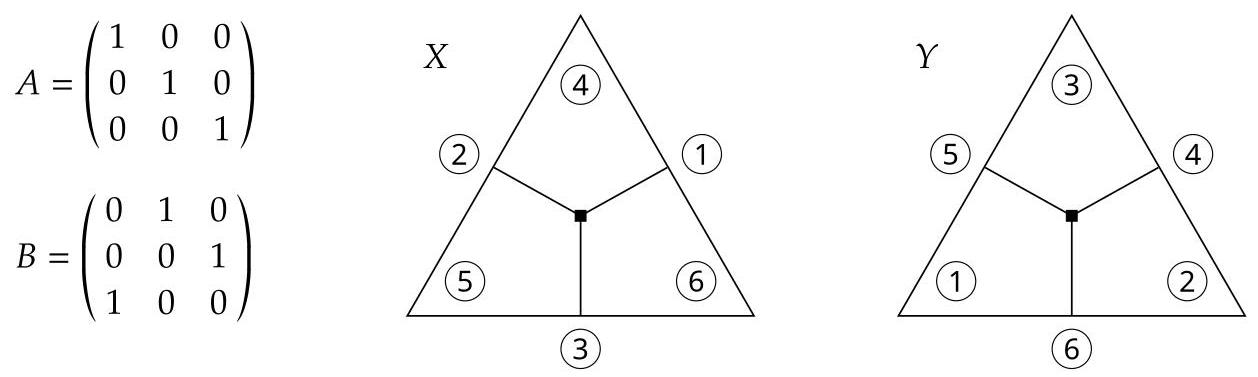
\includegraphics[width=0.9\textwidth]{images/ch09-fig08.jpg}
\caption{一个博弈 $(A, B)$，具有纯最优反应的完整循环\eqref{eq:9.9}。该博弈的唯一均衡是完全混合均衡，用黑色方块标记。}
\label{fig:9.8}
\end{figure}


图\ref{fig:9.8}展示了一个博弈$(A, B)$，其中 \(A\) 是单位矩阵，\(B\) 是对列进行置换后的单位矩阵。因此，相较于图\ref{fig:9.7}，\(X\) 中的最优反应区域形状相同但标签不同。正如最优反应示意图和收益矩阵所示，在这个博弈中存在一个纯最优反应的完整循环：
\begin{equation}  \label{eq:9.9}
\circled{1}\rightarrow  \circled{5} \rightarrow  \circled{2}\rightarrow  \circled{6} \rightarrow \circled{3} \rightarrow  \circled{4} \rightarrow  \circled{1}
\end{equation}

在这个博弈中，除了完全混合均衡（其中 \(x = y = \left( {\frac{1}{3},\frac{1}{3},\frac{1}{3}}\right)\)）外，不存在其他完全标记的混合策略对$(x, y)$。这一点从最优反应示意图可以看出。具体而言，根据式\eqref{eq:9.9}，显然不存在纯策略均衡。进一步，\(X\) 中标签为3、5、6的点 \(x = \left( {\frac{1}{2},\frac{1}{2},0}\right)\) 需要 \(Y\) 中标签为1、2、4的点\(y\)成为均衡的一部分，但 \(Y\) 中没有同时具有标签1和4的点。类似地，\(X\) 中标签为1、4、6的点需要 \(Y\) 中标签为2、3、5的点，但 \(Y\) 中没有同时具有标签2和5的点。\(X\) 中标签为2、4、5的点需要 \(Y\) 中标签为1、3、6的点，但 \(Y\) 中没有同时具有标签3和6的点。

这就引出了一个普遍问题：对于一个非退化博弈，纯最优反应的循环\eqref{eq:9.9}是否意味着该博弈有唯一的混合策略纳什均衡（这对于 \(2 \times  2\) 博弈是成立的）。借助最优反应图，可以轻松回答这个问题。三角形顶点处的纯最优反应由\eqref{eq:9.9}确定。我们从图\ref{fig:9.9}开始分析，首先保持 \(A\)不变，因此最优反应区域 \(Y\left( 1\right)，Y\left( 2\right)\) 和 \(Y\left( 3\right)\) 也不变。\(Y\) 中具有标签1、2、6的点\(y = \left( {\frac{1}{2},\frac{1}{2},0}\right)\)，能否成为某个均衡$(x, y)$的一部分呢？如果可以，则要求 \(x\) 具有标签3、4、5。如果在具有标签3的 \(X\) 的底边上，标签4出现在标签5和6之间，那么这确实是可能的。从最优反应图可知，点\(x = \left( {\frac{2}{3},\frac{1}{3},0}\right)\) 具有标签3、4、5。均衡策略 \(x\) 和 \(y\) 用黑色方块标记，且最优反应图也表明均衡是唯一的。因此，该博弈确实只有一个均衡，尽管它不是完全混合的。

\begin{figure}[htbp]
\centering
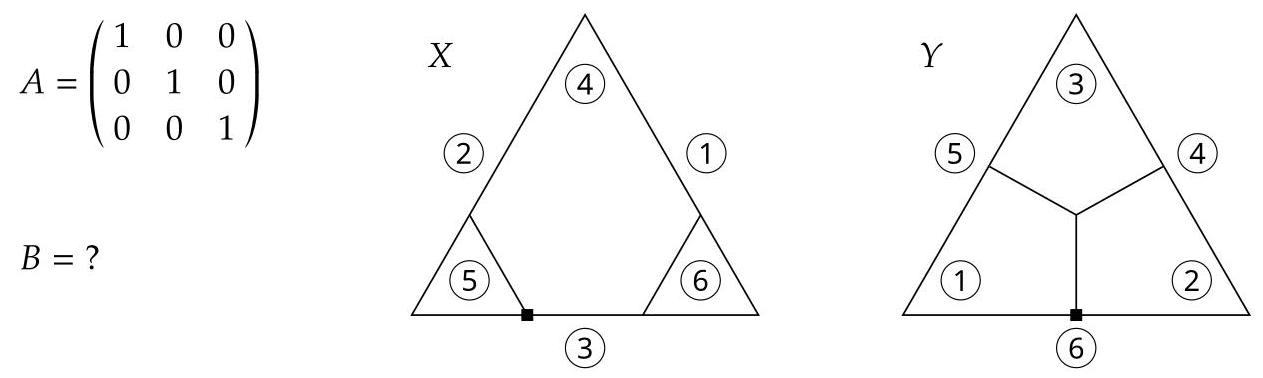
\includegraphics[width=0.9\textwidth]{images/ch09-fig09.jpg}
\caption{一个具有纯最优反应的完整循环\eqref{eq:9.9} 且对于 \(x = \left( {\frac{2}{3},\frac{1}{3},0}\right)\) 和 \(y = \left( {\frac{1}{2},\frac{1}{2},0}\right)\) 有唯一均衡$(x，y)$的博弈的最优反应示意图。收益矩阵 \(B\) 在图\ref{fig:9.10}中构建。}
\label{fig:9.9}
\end{figure}


我们已经先绘制了最优反应图。图\ref{fig:9.10}则展示根据 \(X\) 划分的最优反应区域，构建一个收益矩阵 \(B\)的过程。
\begin{figure}[htbp]
\centering
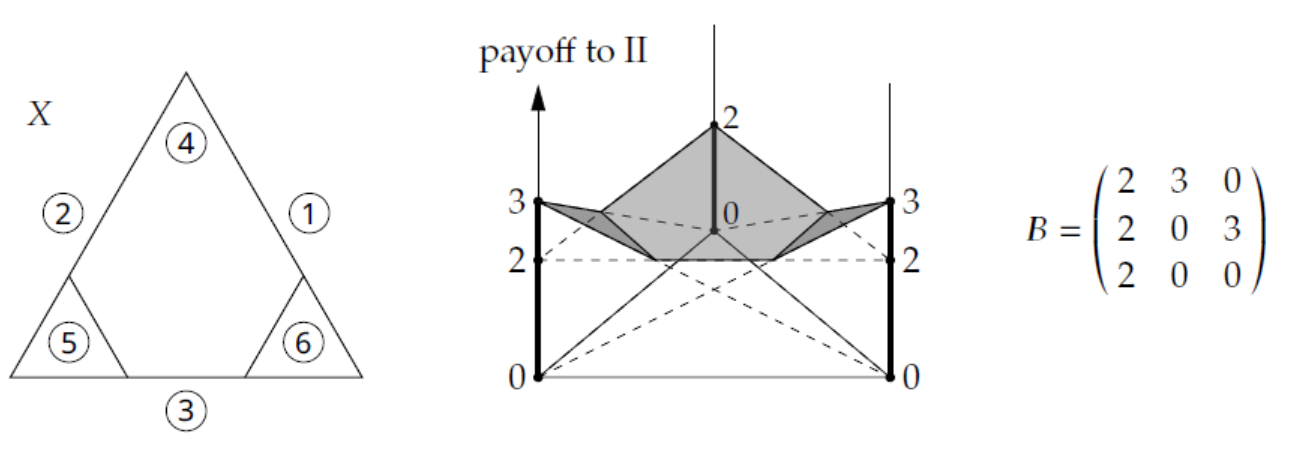
\includegraphics[width=0.9\textwidth]{images/ch09-fig10.png}
\caption{通过合适收益的上包络从左侧的最优反应示意图构建博弈矩阵 \(B\)。第一列4定义了一个常数收益为2的水平面，第二列和第三列5和6分别在角 \({e}_{1}\) 和 \({e}_{2}\) 处有更高的收益3，其他地方为0。}
\label{fig:9.10}
\end{figure}


图\ref{fig:9.11}展示了一个博弈及其最优反应区域，其最优反应区域 \(Y\left( 1\right), Y\left( 2\right), Y\left( 3\right)\) 和收益矩阵 \(A\) 相对于图\ref{fig:9.10}发生了变化。该博弈仍然有纯最优反应的完整循环 \eqref{eq:9.9}，但它有三个均衡。因此，条件 \eqref{eq:9.9}并不意味着有唯一的均衡。借助最优反应示意图，可以比较容易构造出这个反例。

\begin{figure}[htbp]
\centering
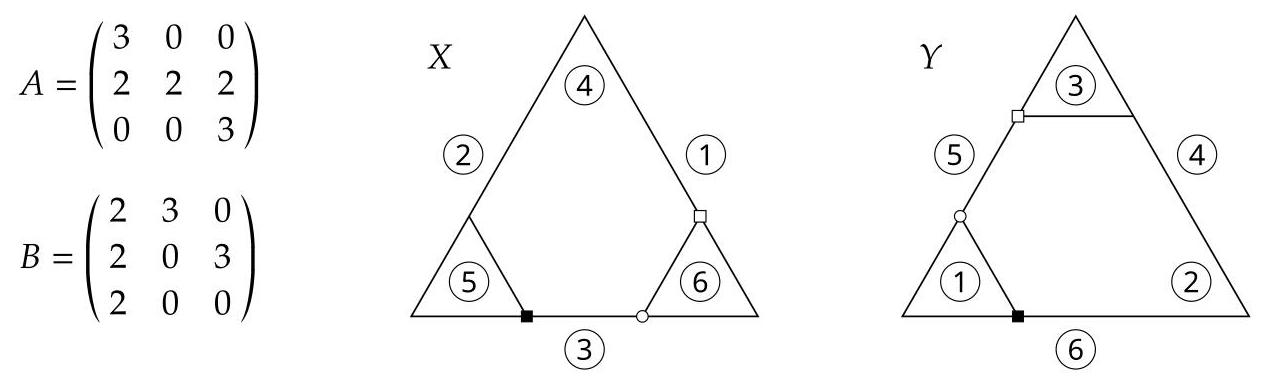
\includegraphics[width=0.9\textwidth]{images/ch09-fig11.jpg}
\caption{一个具有纯最优反应的完整循环(9.9)和多个均衡的博弈。}
\label{fig:9.11}
\end{figure}

图\ref{fig:9.12}展示了一个博弈及其最优反应区域，其中 \(X\) 的划分在性质上处于图\ref{fig:9.8}和图\ref{fig:9.9}之间的过渡状态。根据引理9.3，这是一个退化博弈，因为 \(x = \left( {\frac{1}{2},\frac{1}{2},0}\right)\) 有三个纯最优反应和四个标签3、4、5、6。如果$(x,y)$是一个均衡，则点 \(y\) 只需要两个标签1和2即可。这两个标签定义了 \(Y\left( 1\right)  \cap  Y\left( 2\right)\)，它是 \(Y\) 中端点为 \(\left( {\frac{1}{2},\frac{1}{2},0}\right)\) 和 \(\left( {\frac{1}{3},\frac{1}{3},\frac{1}{3}}\right)\) 的线段。该线段中的任何 \(y\) 都是均衡$(x,y)$的一部分，所以这个博弈有无限个均衡。

\begin{figure}[htbp]
\centering
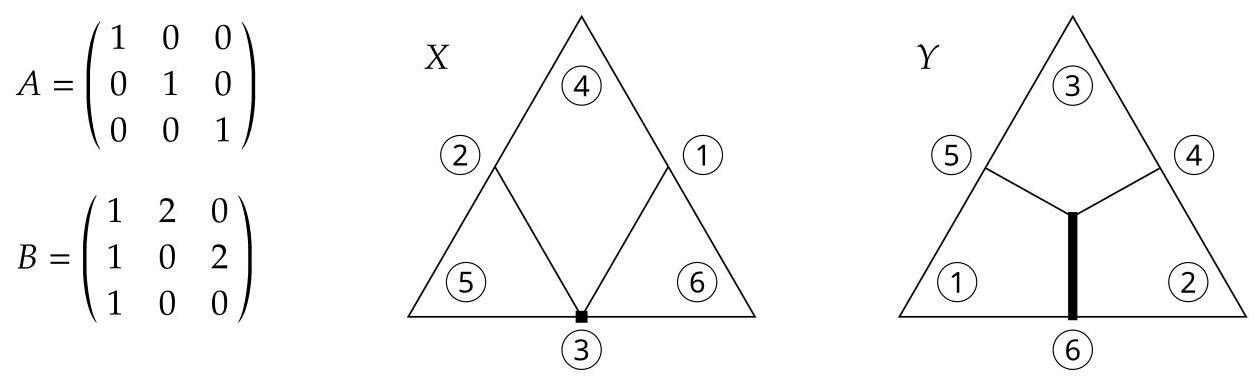
\includegraphics[width=0.9\textwidth]{images/ch09-fig12.jpg}
\caption{一个具有多个均衡线段的退化博弈。}
\label{fig:9.12}
\end{figure}

对于非退化博弈，命题\ref{prop:6.8}指出，均衡 $(x, y)$中的两个均衡策略所混合的纯策略数量相同。对于最优反应图而言，这意味着包含$x$的最小面$X$与包含$y$的最小面$Y$具有相同的维度。如果 $(x,y)$是纯策略均衡，这个面就是一个顶点；如果$x$和$y$仅混合两种纯策略，这个面就是一条边；如果二者混合三种策略，这个面就是一个三角形（对于更大的博弈，这个面的维度更高）。到目前为止所看到的示意图都是这种情况，但图\ref{fig:9.12}中的退化博弈并非如此。在该图中，\(X\)下边缘的均衡策略 \(x = \left( {\frac{1}{2},\frac{1}{2},0}\right)\)与三角形$Y$内部的任意点 \(y = \left( {\alpha,\frac{1}{2} - \frac{\alpha }{2},\frac{1}{2} - \frac{\alpha }{2}}\right)\)（其中$0 < \alpha  \leq  \frac{1}{3}$）构成一个均衡 $(x, y)$。


\section{策略等价}  \label{sec9.5}
在构建一个博弈的最优反应图时，考虑另一个具有相同示意图的博弈通常会更简单。这样的两个博弈被称为策略等价。下面定义一般的 $N$人博弈的策略等价。

\begin{definition} \label{def:9.5}  %定义9.5
    给定一个$N$人策略型博弈$G$。对于任意参与人 $i = 1, \ldots, N$，其策略集为 $S_i$，其在策略组$s$下收益为 $u_i(s)$，混合策略为$
\sigma_i \in X_i = \Delta(S_i)$，除$i$之外的混合策略组为$\sigma_{-i} \in X_{-i} = \prod_{k \neq i} X_k$。设 $\widehat{G}$ 是另一个具有相同策略集的博弈，其参与人 $i$ 的收益函数为 $\widehat{u}_i$。那么，如果对于所有的$i = 1, \ldots, N$ 和所有 $\sigma_{-i} \in X_{-i}$，在 $G$ 中任意策略 $s_i \in S_i$ 是对 $\sigma_{-i}$ 的最优反应，当且仅当 在 $\widehat{G}$ 中$s_i$ 也是对 $\sigma_{-i}$ 的最优反应时，则称 $G$ 与 $\widehat{G}$ 是策略等价的。
\end{definition}


因此，两个 \( m  \times  n \)双矩阵博弈的策略等价意味着：在一个博弈中，任何行$i$是对参与人II的混合策略$y$的最优反应，当且仅当在另一个博弈中行$i$也是对$y$的最优反应；类似地，在一个博弈中，任何列$j$是对参与人I的混合策略$x$的最优反应，当且仅当在另一个博弈中列$j$也是对 $x$的最优反应。这等价于说，两个博弈具有相同的最优反应区域 $Y(j)$和$Y(i)$（如式\eqref{eq:9.3}所定义），即具有相同的最优反应示意图。


如图\ref{fig:6.10}和图\ref{fig:9.1}所示，图\ref{fig:6.7}右侧的博弈与图\ref{fig:9.1}中的博弈是策略等价的。这两个博弈对于参与人II而言具有相同的收益矩阵 \(B\)，且第二个博弈中的收益矩阵 \(A\) 是由第一个博弈的收益矩阵\(A\)的第一列中每个元素加上常数1而得到。这通常是一种构造策略等价博弈的方法。考虑一个双矩阵博弈$(A,B)$，并给 \(A\) 的第 \(j\) 列的每个元素加上一个常数 \(\alpha\)。如果参与人II采用混合策略 \(y\)，即第 \(j\) 列的概率为 \({y}_{j}\)，那么第 \(i\) 行的期望收益就从 \({\left( Ay\right) }_{i}\) 变为 \({\left( Ay\right) }_{i} + \alpha {y}_{j}\)。也就是说，所有这些期望收益都改变了相同的量 \(\alpha {y}_{j}\)。尽管这依赖于 \(y\)，但它并不会改变哪些行 \(i\) 具有最大收益，因此也不会改变参与人I对 \(y\) 的最优反应。我们将这种给行参与人收益的某一列加上一个常数的收益变化称为博弈的列移位。

在\(N\) 人博弈中，列移位也是一个通用术语，其假设所考虑参与人的纯策略暂时被排列为行，而其他 \(N - 1\) 个参与人的任何部分策略组合对应于一列。例如，练习~\ref{exer:3.2} 中的三人博弈将参与人I的策略作为行，将参与人II和参与人III的部分纯策略组合作为列。需要注意，在双矩阵博弈$(A,B)$中，参与人II的列移位意味着给参与人II的收益矩阵 \(B\) 的某一行加上一个常数。



\begin{definition}\label{def:9.6}  %定义9.6
考虑如定义\ref{def:9.5}所述的一个 \(N\) 人博弈 \(G\)。设\(i = 1,\ldots,N\) 为任意一个参与人，\({a}_{i}\left( {s}_{-i}\right)  \in  \mathbb{R}\) 为对应于其他 \(N - 1\) 个参与人的纯策略组合 \({s}_{-i}\) 的一个常数。定义参与人 \(i\) 的一个新的效用函数 \({\widehat{u}}_{i}\)：
\[
{\widehat{u}}_{i}\left( {{s}_{i},{s}_{-i}}\right)  = {u}_{i}\left( {{s}_{i},{s}_{-i}}\right)  + {a}_{i}\left( {s}_{-i}\right)
\]
这种变换称为参与人 \(i\) 的列移位。
\end{definition}


\begin{proposition}\label{prop:9.7}   %命题9.7
考虑如定义~\ref{def:9.6} 所述的一个 \(N\) 人博弈 \(G\)，参与人 \(i\) 通过列移位获得了一个新的效用函数 \({\widehat{u}}_{i}\)。那么，用 \({\widehat{u}}_{i}\) 替代 \({u}_{i}\) 后的博弈 \(\widehat{G}\) 与 \(G\) 是策略等价的。
\end{proposition}

\begin{proof}
采用定义\ref{def:9.6}中的符号，设 \({s}_{i} \in  {S}_{i}\) 是参与人 \(i\) 的一个策略，\({\sigma }_{-i}\) 是其他参与人的一个混合策略组合。那么，在 \(G\) 中参与人 \(i\) 的期望收益是 \({U}_{i}\left( {{s}_{i},{\sigma }_{-i}}\right)\)，在 \(\widehat{G}\) 中参与人 \(i\) 的期望收益是 \({U}_{i}\left( {{s}_{i},{\sigma }_{-i}}\right)  + {a}_{i}\left( {s}_{-i}\right) \mathop{\prod }\limits_{{k = 1,k \neq  i}}^{N}{\sigma }_{k}\left( {s}_{k}\right)\)。对于后者，因为额外相加的项不依赖于 \({s}_{i}\)，所以在确定参与人 $i$ 对 $\sigma_{-i}$ 的最优反应时，最大值对应的$s_i \in S_i$不会受到列移位的影响。也就是说，\(G\) 和 \(\widehat{G}\) 中对 \({\sigma }_{-i}\) 的最优反应是相同的。
\end{proof}


列移位可能意味着对所有“列”增加同一个常数，从而使所有收益都增加同一个常数。这仅仅改变了参与人效用函数的原点，因此始终表示相同的偏好。此外，参与人的收益可以通过乘以一个正常数（该常数不能随列变化）来进行缩放，这种变换显然会产生一个策略等价的博弈。然而，即使一个博弈不能通过缩放和列移位从另一个博弈得到，两个博弈也可能是策略等价的。考虑 \(3 \times  2\) 博弈 $(A, B)$ 和 $({\widehat{A},B})$，其中
\begin{equation}  \label{eq:9.10}
 A = \left( \begin{array}{cc} 2 & 0 \\  1 & 2 \\  0 & 3 \end{array}\right)，\;
 \widehat{A} = \left( \begin{array}{cc} 2 & 0 \\  1 & 2 \\ \frac{1}{2} & \frac{5}{2} \end{array}\right)
\end{equation}
以及任何 \(B\)，例如如式\eqref{eq:9.1} 中所示。图\ref{fig:9.13} 中两个博弈的上包络图表明，这两个博弈是策略等价的，因为它们具有相同的最优反应区域 \(Y\left( 1\right), Y\left( 2\right), Y\left( 3\right)\)。特别地，当 \(y = \left( {\frac{1}{2},\frac{1}{2}}\right)\) 时，第 2 行和第 3 行之间的无差异，且这两行都是最优反应。然而， \(\widehat{A}\) 不能通过缩放和列移位从 \(A\) 得到：\(A\) 和 \(\widehat{A}\) 第一列的前两个元素是相同的，即 2 和 1，这确定了第一列收益的“效用尺度”，因此不能对该列应用任何缩放或加法移位，但该列的第三个元素在 \(A\) 和 \(\widehat{A}\) 中却不同。

\begin{figure}[htbp]
\centering
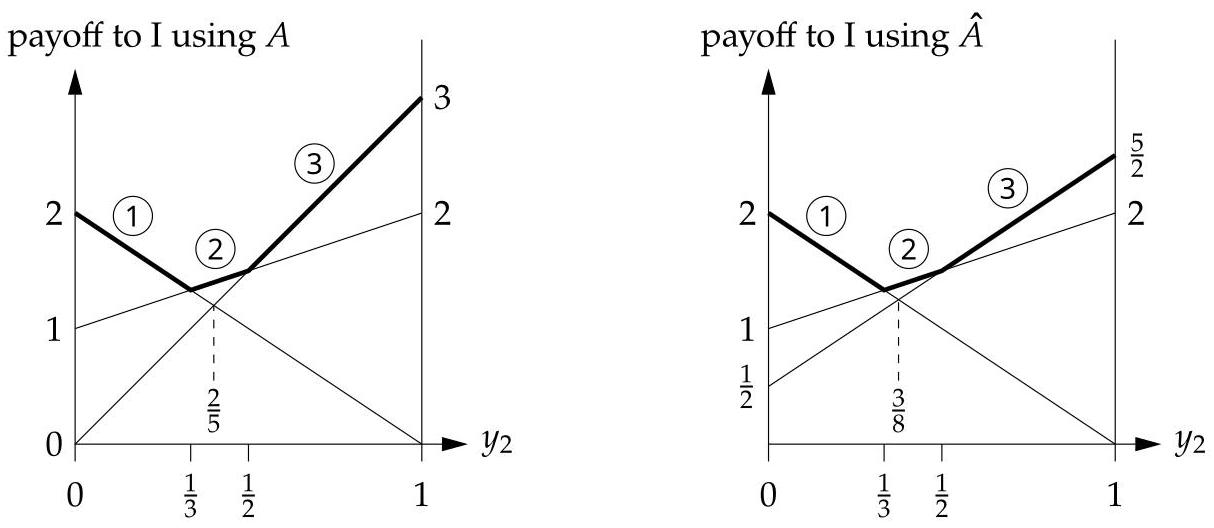
\includegraphics[width=0.9\textwidth]{images/ch09-fig13.jpg}
\caption{针对式\eqref{eq:9.10} 中收益矩阵 \(A\) 和 \(\widehat{A}\)，参与人 I 相对于 \(\left( {{y}_{1},{y}_{2}}\right)\) 的期望收益的上包络图，这些矩阵定义了策略等价但不是强策略等价的博弈 $(A, B)$ 和 \(( {\widehat{A},B})\)。}
\label{fig:9.13}
\end{figure}

请注意，我们仅根据最优反应来定义策略等价，而最优反应与均衡相关。式\eqref{eq:9.10}中 \(A\) 和 \(\widehat{A}\) 的第 1 行和第 3 行没有相同的无差异点。具体而言，对于 \(A\)，当 \(y = \left( {\frac{3}{5},\frac{2}{5}}\right)\) 时，这两行的收益都为 \(\frac{6}{5}\)；对于 \(\widehat{A}\)，当 \(y = \left( {\frac{5}{8},\frac{3}{8}}\right)\) 时，这两行的收益都为 \(\frac{5}{4}\)。然而，在这两种情况下，第 1 行和第 3 行都不在上包络上，因为第 2 行的收益更高，如图\ref{fig:9.13} 所示。


一个更强的定义（采用定义\ref{def:9.5} 中的符号）是：如果对于所有参与人 \(i = 1,\ldots,N\)和所有 \({\sigma }_{-i} \in  {X}_{-i}\) 以及 \({S}_{i}\) 中的任意两个策略 \({s}_{i}\) 和 \({s}_{i}^{\prime }\)，有
\begin{equation}  \label{eq:9.11}
{u}_{i}\left( {{s}_{i},{\sigma }_{-i}}\right)  \geq  {u}_{i}\left( {{s}_{i}^{\prime },{\sigma }_{-i}}\right) \; \Leftrightarrow  \;{\widehat{u}}_{i}\left( {{s}_{i},{\sigma }_{-i}}\right)  \geq  {\widehat{u}}_{i}\left( {{s}_{i}^{\prime },{\sigma }_{-i}}\right),
\end{equation} 
则称$G$ 与 $\widehat{G}$ 是强策略等价的。

显然，强策略等价意味着策略等价；任何列移位都意味着强策略等价，因为{\color{red}命题\ref{prop:9.7}}的证明仍然适用。然而，反之则不成立，例 \eqref{eq:9.10} 可以说明这一点。具体而言，当 \(i\) 为行参与人， \({\sigma }_{-i} = y = \left( {{0.61},{0.39}}\right)\) 以及 \({s}_{i}\) 和 \({s}_{i}^{\prime }\) 分别取第 1 行和第 3 行时，式\eqref{eq:9.11}不成立。


我们通过一个例子说明如何利用列移位简化最优反应图的绘制。考虑 \(3 \times  3\) 博弈 $(A, B)$，其中
\begin{equation}  \label{eq:9.12}
A = \left( \begin{array}{rrr} 0 & 3 & 0 \\  1 & 0 & 1 \\   - 3 & 4 & 5 \end{array}\right)，\;B = \left( \begin{array}{rrr} 0 & 1 &  - 2 \\  2 & 0 & 3 \\  2 & 1 & 0 \end{array}\right).
\end{equation} 


我们给 \(A\) 的第一列和第三列加上常数 3，给 \(B\) 的第一行加上常数 2。根据命题~\ref{prop:9.7}，这产生了一个与 $(A, B)$ 策略等价的新博弈 \(( {\widehat{A},\widehat{B}})\)，其中
\begin{equation}  \label{eq:9.13}
\widehat{A} = \left( \begin{array}{lll} 3 & 3 & 3 \\  4 & 0 & 4 \\  0 & 4 & 8 \end{array}\right)，\;\widehat{B} = \left( \begin{array}{lll} 2 & 3 & 0 \\  2 & 0 & 3 \\  2 & 1 & 0 \end{array}\right).
\end{equation} 

博弈 \(( {\widehat{A},\widehat{B}})\) 具有图\ref{fig:9.14} 所示的最优反应图，进而博弈 $(A, B)$有相同的示意图。由于这些图可以通过三个期望收益平面的上包络来较为容易地可视化，因此能够直观地理解这些划分结构。这三个平面分别由每个三角形顶点处的三个支柱点确定，其中第一个策略对应的平面上的支柱点高度相同，因此该平面是水平的。这已在图\ref{fig:9.10} 中展示。图\ref{fig:9.10} 中的矩阵 \(B\) 与 \(\widehat{B}\) 几乎相同，因此图\ref{fig:9.10}与图\ref{fig:9.14}对 \(X\) 的细分几乎相同。


\begin{figure}[htbp]
\centering
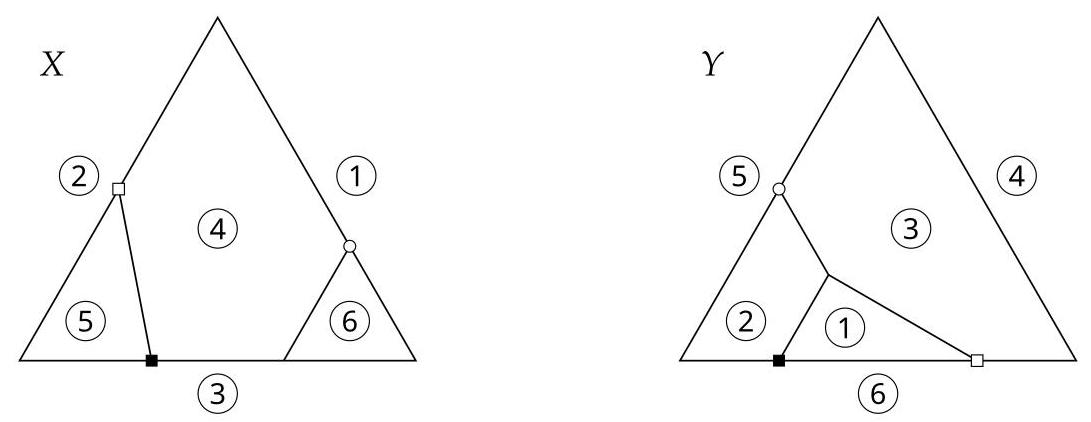
\includegraphics[width=0.8\textwidth]{images/ch09-fig14.jpg}
\caption{博弈\eqref{eq:9.12} 和 \eqref{eq:9.13} 的最优反应图。这些博弈有相同的三个均衡，即 \(\left( {\left( {\frac{2}{3},\frac{1}{3},0}\right), \left( {\frac{3}{4},\frac{1}{4},0}\right) }\right)\)（黑色方块）、 \(\left( {\left( {\frac{1}{2},0,\frac{1}{2}}\right), \left( {\frac{1}{4},\frac{3}{4},0}\right) }\right)\)（白色方块）和 \(\left( {\left( {0,\frac{2}{3},\frac{1}{3}}\right), \left( {\frac{1}{2},0,\frac{1}{2}}\right) }\right)\)（白色圆圈）。}
\label{fig:9.14}
\end{figure}


将 \(Y\) 细分为最优反应区域 \(Y\left( 1\right), Y\left( 2\right), Y\left( 3\right)\)的方法类似于图\ref{fig:9.10}，即通过考虑期望收益的三个平面的上包络来获得。我们还介绍另一种可以直接应用于三角形 \(Y\) 的方法，而无需考虑第三个维度。对于原始博弈 $(A, B)$，最优反应区域是通过比较每行的期望收益来确定：
\begin{equation}  \label{eq:9.14}
\begin{aligned}
Y(1) = \{ \left( y_1, y_2, y_3 \right) \in Y \mid & ~~ 3y_2 \geq y_1 + y_3, \\
   & ~~ 3y_2 \geq -3y_1 + 4y_2 + 5y_3 \}, \\
Y(2) = \{ \left( y_1, y_2, y_3 \right) \in Y \mid & ~~ y_1 + y_3 \geq 3y_2, \\
   & ~~ y_1 + y_3 \geq -3y_1 + 4y_2 + 5y_3 \}, \\
Y(3) = \{ \left( y_1, y_2, y_3 \right) \in Y \mid & ~~ -3y_1 + 4y_2 + 5y_3 \geq 3y_2, \\
   & ~~-3y_1 + 4y_2 + 5y_3 \geq y_1 + y_3\}.
\end{aligned}
\end{equation}


对于博弈 \(( {\widehat{A},\widehat{B}})\)，这些条件是
\begin{equation}   \label{eq:9.15}
\begin{aligned}
Y(1) =  \{ \left( y_1, y_2, y_3 \right) \in Y \mid &~~  3y_1 + 3y_2 + 3y_3 \geq 4y_1 + 4y_3, \\
     & ~~ 3y_1 + 3y_2 + 3y_3 \geq 4y_2 + 8y_3 \}, \\
Y(2) = \{ \left( y_1, y_2, y_3 \right) \in Y \mid & ~~ 4y_1 + 4y_3 \geq 3y_1 + 3y_2 + 3y_3, \\
     & ~~ 4y_1 + 4y_3 \geq 4y_2 + 8y_3 \}, \\
Y(3) = \{ \left( y_1, y_2, y_3 \right) \in Y \mid & ~~ 4y_2 + 8y_3 \geq 3y_1 + 3y_2 + 3y_3, \\
     & ~~ 4y_2 + 8y_3 \geq 4y_1 + 4y_3 \}.
\end{aligned}
\end{equation}


与命题~\ref{prop:9.7} 一致，上述两组条件是完全等价的，因为项 \(3{y}_{1} + 3{y}_{3}\) 被加到每个不等式的两边。这对应于通过给 \(A\) 的第一列和第三列加上常数 3 以得到 \(\widehat{A}\) 的列移位。

\begin{figure}[htbp]
\centering
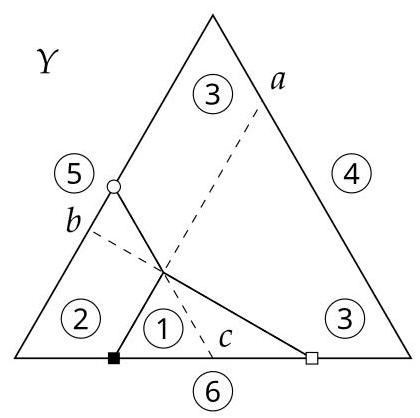
\includegraphics[width=0.35\textwidth]{images/ch09-fig15.jpg}
\caption{在平面中对 \(Y\) 进行细分的构建，无需三维上包络。}
\label{fig:9.15}
\end{figure}


我们现在考虑每两行之间的无差异，并将它们写成如下形式:
\begin{equation}  \label{eq:9.16}
\begin{aligned}
\circled{1} \sim \circled{2} : & \quad 3y_2 = y_1 + y_3, \\
\circled{1} \sim \circled{3} : & \quad 3y_1 = y_2 + 5y_3, \\
\circled{2} \sim \circled{3} : & \quad 4y_2 + 4y_3 = 4y_1.
\end{aligned}
\end{equation}

式 \eqref{eq:9.16} 中的方程组是通过以下步骤得到的：首先，将式 \eqref{eq:9.14} 或 \eqref{eq:9.15} 中的不等式转化为等式；然后，整理${y}_{1}$、${y}_{2}$ 和 ${y}_{3}$ 的系数，确保每个变量仅以正系数出现在方程的一侧（如果某个变量在两侧的系数相同，则该变量可以消去；不过在这里并不存在这种情况）。对于博弈 \eqref{eq:9.1}，在式 \eqref{eq:9.4} 中已做类似处理，从而便利地确定了两个最优反应区域$X(4)$和$X(5)$ 的公共线段。


回到本例，可以通过扩展上述方法找到三个最优反应区域 \(Y(1),Y(2)\) 和 \(Y(3)\)，如图\ref{fig:9.15}所示。式\eqref{eq:9.16}中的第一个方程表示行1和行2具有相同期望收益的位置。该方程中出现了所有三个变量 \({y}_{1},{y}_{2},{y}_{3}\)，其中 \({y}_{1}\) 在左侧，\({y}_{2}\) 和 \({y}_{3}\) 在右侧。令 \({y}_{3} = 0\)，则得到解 \(y = \left( {\frac{3}{4},\frac{1}{4},0}\right)\)，在图\ref{fig:9.15}中用黑色方块表示；令 \({y}_{1} = 0\)，则得到另一个解 \(y = \left( {0,\frac{1}{4},\frac{3}{4}}\right)\)，在图中表示为点 \(a\)。连接这两个点的线段将 \(Y(1)\) 和 \(Y(2)\) 分开。为确定标签1和2应绘制在该线段的哪一侧，可以先明确参与人I针对参与人II的纯策略的最优反应：针对 \({e}_{1}\) 的最优反应是行2，针对 \({e}_{2}\) 和 \({e}_{3}\) 的最优反应是行3，这些信息通过三角形顶点处的标签表示出来。

类似地，式\eqref{eq:9.16}中第二个方程的极端解是：当 \({y}_{3} = 0\) 时 \(y =\)  \(\left( {\frac{1}{4},\frac{3}{4},0}\right)\)，在图\ref{fig:9.15}中用白色方块表示；当 \({y}_{2} = 0\) 时 \(y = \left( {\frac{5}{8},0,\frac{3}{8}}\right)\)，即图中的点$b$。对于式\eqref{eq:9.16}中的第三个方程，其极端解为 \( \left( {\frac{1}{2},\frac{1}{2},0}\right)\) 和 \(\left( {\frac{1}{2},0,\frac{1}{2}}\right)\)，其中前者在图中用点 $c$表示，后者用白色圆圈表示（注意到，该方程的任意解都有 \({y}_{1} = \frac{1}{2}\)）。三个最优反应区域在 \(Y\) 的内部有一个公共点，该点可以计算得出为 \(\left( {\frac{1}{2},\frac{1}{4},\frac{1}{4}}\right)\)（尽管其精确位置与最优反应图的定性形状无关）。


为了确定博弈\eqref{eq:9.12}的均衡，不必精确地构造图\ref{fig:9.14}中的最优反应图，只需展示各三角形中最优反应区域的交汇位置，以确定具有三个标签的点。三个均衡仍然像之前一样用相应的符号表示。

\begin{figure}[htbp]
\centering
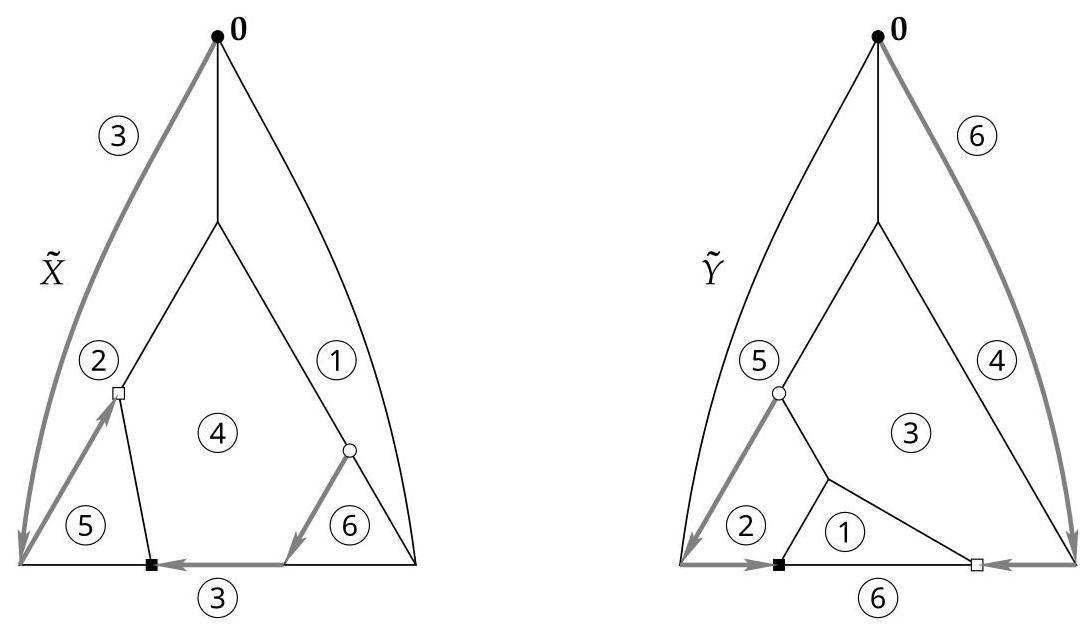
\includegraphics[width=0.8\textwidth]{images/ch09-fig16.jpg}
\caption{博弈\eqref{eq:9.12}中缺失标签1的莱姆基 - 豪森路径，如\eqref{eq:9.17}和\eqref{eq:9.18}所示。}
\label{fig:9.16}
\end{figure}


图\ref{fig:9.16}展示了博弈\eqref{eq:9.12}中针对缺失标签1的莱姆基-豪森路径，该路径基于图\ref{fig:9.14}中的最优反应图。如前所述，通过在 $X$ 和 $Y$ 中分别加入点 $\mathbf{0}$，并将其分别与 $X$ 和 $Y$ 的各顶点用边连接，得到图 $\widetilde{X}$ 和 $\widetilde{Y}$。为避免图示过于杂乱，我们仅通过标签集合来表示 $\widetilde{X} \times \widetilde{Y}$ 中的点对 $(x,y)$，并用相应符号表示均衡。这些路径如下所示：
\begin{equation} \label{eq:9.17}
\adjustbox{max width=\textwidth}{
\begin{tabular}{ccc}
\hline
$(x,y)$ & 标签 & 去掉的标签 \\
\hline
$\bullet$ & $123,456$ &  \(\widetilde{X}\) 中的标签1 \\
 & $235,456$ & \(\widetilde{Y}\) 中的标签5 \\
 & $235,{\color{red}346}$ &  \(\widetilde{X}\)中的标签3  \\
 & $245,{\color{red}346}$ &  \(\widetilde{Y}\)中的标签4 \\
$\square$ & $245,136$ & （\(\widetilde{Y}\)中找到了标签1） \\
\hline
\end{tabular}
}
\end{equation}
和
\begin{equation}  \label{eq:9.18}
\adjustbox{max width=\textwidth}{
\begin{tabular}{ccc}
\hline
$(x,y)$ & 标签 & 去掉的标签 \\
\hline
$\circ$ & $146,235$ & $\widetilde{X}$中的标签1 \\
 & $346,235$ & $\widetilde{Y}$中的标签3 \\
 & $346,256$ & $\widetilde{X}$中的标签6 \\
 & $345,256$ & $\widetilde{Y}$中的标签5 \\
$\blacksquare$ & $345,126$ & （ $\widetilde{Y}$中找到了标签1） \\
\hline
\end{tabular}
}
\end{equation}



针对每个缺失标签，找出图~\ref{fig:9.16}中的莱姆基 - 豪森路径是一个有益的练习。例如，图~\ref{fig:9.16}中用白色圆圈标记的均衡 \(\left( {\left( {0,\frac{2}{3},\frac{1}{3}}\right),\left( {\frac{1}{2},0,\frac{1}{2}}\right) }\right)\) 是从人工均衡$(\mathbf{0},\mathbf{0})$出发，针对缺失标签3找到的，因此它不同于在缺失标签 1 时所找到的均衡。以该白色圆圈作为起点，缺失标签1的莱姆基 - 豪森路径如\eqref{eq:9.18}所示，由此能找到第三个均衡。通过考虑所有可能的缺失标签，可以构建一个能够来回遍历的莱姆基 - 豪森路径组成的网络。然而，这个网络可能不是连通的，因此从人工均衡出发时，并不能保证找到所有均衡；参见练习~\ref{exer:9.1}。



\section{最优反应多面体和有界多面体}  \label{sec9.6}



如前两节所示，最优反应图有助于直观呈现\(3 \times  3\)博弈中均衡的结构。同时，它也是在更大规模双矩阵博弈中寻找均衡的一般算法的重要基础。这些算法（包括莱姆基 - 豪森算法）都建立在上包络图的基础之上。上包络图可以通过适当定义的最优反应多面体进行一般化描述，本节将对此进行解释。

如前所述，\({\mathbb{R}}^{d}\) 中的超平面 \(H\) 是一个集合 \(H = \left\{  {z \in  {\mathbb{R}}^{d} \mid  {v}^{\top }z = \alpha }\right\}\)，其中 \(v\)是\({\mathbb{R}}^{d}\) 中的非零法向量，\(\alpha\)是实数。相应的半空间定义为 \(\left\{  {z \in  {\mathbb{R}}^{d} \mid  {v}^{\top }z \leq  \alpha }\right\}\)。多面体是有限个半空间的交集。如果多面体 \(S\) 是 \(n\) 个半空间 \(\left\{  {z \in  {\mathbb{R}}^{d} \mid  {c}_{i}^{\top }z \leq  {q}_{i}}\right\}\) 的交集，其中 \({c}_{i} \in  {\mathbb{R}}^{d}\) 且 \({q}_{i} \in  \mathbb{R}\) （对于 \(i = 1,\ldots,n\) ），那么它可以写成
\begin{equation}  \label{eq:9.19}
S = \left\{  {z \in  {\mathbb{R}}^{d} \mid  {Cz} \leq  q}\right\}
\end{equation}
其中，\(C\)为\(n \times  d\) 矩阵和 \(q \in  {\mathbb{R}}^{n}\)，并且\({C}^{\top } = \left\lbrack  {{c}_{1}\cdots {c}_{n}}\right\rbrack\)，即 \({c}_{i}^{\top }\) 是 \(C\) 的第 \(i\) 行。

如果 \(z \in  S\) 且 \({c}_{i}^{\top }z = {q}_{i}\)，那么称式\eqref{eq:9.19} 中的第 \(i\) 个不等式 \({c}_{i}^{\top }z \leq  {q}_{i}\) 在 \(z\) 处是紧的（即等号成立）。\(S\) 的一个面 \(F\)可以通过要求式\eqref{eq:9.19}  中\(n\)个不等式中的某些不等式取等号得到（因此，\(F\) 可能为空集)。也就是说，对于某个集合 \(T \subseteq  \{ 1,\ldots,n\}\)，有\(F = \left\{  {z \in  S \mid  {c}_{i}^{\top }z = {q}_{i}}\right.\) \mbox{对于} \(\left. {i \in  T}\right\}\)。选择 \(T\) 的方式有 \({2}^{n}\) 种（其中一些可能定义相同的面 \(F\)），因此面的数量是有限的。如果这个面由单个点组成，那么这个点被称为多面体的顶点。有边界的多面体称为有界多面体。可以证明，每个有界多面体都是其顶点的凸包，这与我们之前将有界多面体定义为 \({\mathbb{R}}^{d}\) 中有限点集的凸包是一致的。


混合策略集 \(X\) 和 \(Y\) （见式\eqref{eq:6.6}）是有界多面体，因为它们是有界的，并且由多个线性不等式和一个线性方程定义（任何方程 \({v}^{\top }z = \alpha\) 都可以写成两个不等式 \({v}^{\top }z \leq  \alpha\) 和 \(- {v}^{\top }z \leq   - \alpha\)）。


作为本节的核心概念，对于一个 \(m \times  n\) 双矩阵博弈$(A, B)$，我们考虑参与人 I 的最优反应多面体 \(\bar{P}\) 和参与人 II 的最优反应多面体 \(\bar{Q}\)如下：
\begin{equation}
\label{eq:9.20}
\begin{aligned}
\bar{P} 
&= \left\{ (x,v) \in X \times \mathbb{R} \mid B^{\top}x \le \mathbf{1}v \right\}, \\
\bar{Q} 
&= \left\{ (y,u) \in Y \times \mathbb{R} \mid Ay \le \mathbf{1}u \right\}.
\end{aligned}
\end{equation}

对于式\eqref{eq:9.1}所示的博弈，\(\bar{P}\) 中的不等式 \({B}^{\top }x \leq  \mathbf{1}v\) （其中 \(x \in  X\)）为：
\begin{equation}
\label{eq:9.21}
\begin{aligned}
2x_1 + 4x_3 &\le v, \\
x_2 + x_3 &\le v.
\end{aligned}
\end{equation}
同时，\(\bar{Q}\)中的不等式 \({Ay} \leq  {1u}\) （其中\(y \in  Y\)）为：
\begin{equation}
\label{eq:9.22}
\begin{aligned}
2y_1 &\le u, \\
y_1 + 2y_2 &\le u, \\
3y_2 &\le u.
\end{aligned}
\end{equation}

它们在图\ref{fig:9.2} 和图\ref{fig:9.1} 的上包络图中有所展示，其中 \(v\) 和 \(u\) 分别不小于参与人 II 和参与人 I 的收益（因为 \(v\) 和 \(u\) 没有上界，所以 \(\bar{P}\) 和 \(\bar{Q}\) 是多面体但不是有界多面体）。一旦\eqref{eq:9.21}  和 \eqref{eq:9.22} 中的至少一个不等式是紧的， \(v\) 和 \(u\) 就等于最优反应收益，因为它们不能取更低的值。也就是说，对于给定的 \(x \in  X\) 和 \(y \in  Y\)，
\begin{align*}
\min \{ v \mid (x,v) \in \bar{P} \} 
&= \max \left\{ (B^{\top} x)_j \mid 1 \le j \le n \right\}, \\
\min \{ u \mid (y,u) \in \bar{Q} \} 
&= \max \left\{ (Ay)_i \mid 1 \le i \le m \right\}.
\end{align*}

上述正是我们熟悉的期望收益上包络的定义。假设 \({B}^{\top }x \leq  \mathbf{1}v\) 中的至少一个不等式是紧的（该条件将 \(v\) 确定为对 \(x\) 的最优反应收益），\({B}^{\top }x \leq  \mathbf{1}v\) 中的紧不等式对应于对 \(x\) 的纯最优反应。类似地，\({Ay} \leq  \mathbf{1}u\) 中的紧不等式（如果至少有一个是紧的）对应于对 \(y\) 的纯最优反应。


因此，我们可以将式\eqref{eq:9.2}中表示参与人纯策略 \(1,\ldots,m + n\) 的标签，与 \(\bar{P}\) 和 \(\bar{Q}\) 中的紧不等式对应起来。设 \(\left( {x,v}\right)  \in  \bar{P}\)，其中 \(v\) 是对 \(x\) 的最优反应收益；设 \(\left( {y,u}\right)  \in  \bar{Q}\)，其中 \(u\) 是对 \(y\) 的最优反应收益，并令 \(1 \leq  i \leq  m\) 和 \(1 \leq  j \leq  n\)。那么，根据定义 \ref{def:9.1}，
\begin{equation}  \label{eq:9.23}
\begin{aligned}
x\text{ 具有标签 }i & \Leftrightarrow  {x}_{i} = 0, \\
x\text{ 具有标签 }m + j\; & \Leftrightarrow  \;{\left( {B}^{\top }x\right) }_{j} = v, \\
y\text{ 具有标签 }i\; & \Leftrightarrow  \;{\left( Ay\right) }_{i} = u, \\
y\text{ 具有标签 }m + j\; & \Leftrightarrow  \;{y}_{j} = 0.
\end{aligned}
\end{equation}


因此，我们可以将定理 \ref{theo:9.2}  重新表述如下。

\begin{corollary}  \label{coro:9.8}  %推论 9.8
设 \(\left( {x,v}\right)  \in  \bar{P}\) 和 \(\left( {y,u}\right)  \in  \bar{Q}\)。那么，$(x, y)$ 是 $(A, B)$ 的一个均衡，且\(u\) 和 \(v\)分别是参与人 I 和II 的均衡收益，当且仅当 $(x, y)$ 是完全标记的。
\end{corollary}


在定义 ~\ref{def:9.1} 中，标签是根据式\eqref{eq:9.3} 中的最优反应区域 \(Y\left( i\right)\) 和 \(X\left( j\right)\)，以及式\eqref{eq:9.5}中 \(X\) 和 \(Y\) 的零面来定义的。最优反应区域是有界多面体，例如 式\eqref{eq:9.14}所示的情况。最优反应区域在低维度中（特别是作为三角形的子集）便于绘制；相比之下，通过最优反应多面体 \(\bar{P}\) 和 \(\bar{Q}\) 的面来定义标签时，只需为每个标签对应一个紧约束，即通过在另一个参与人的收益 \(v\) 或 \(u\) 上增加一个维度来实现。


现在，我们通过消除这些收益变量，并将混合策略 \(x\) 和 \(y\) 替换为任意非负向量，从而简化最优反应多面体。设
\begin{equation}
\label{eq:9.24}
\begin{aligned}
P & = \left\{  {x \in  {\mathbb{R}}^{m} \mid  x \geq  \mathbf{0},{B}^{\top }x \leq  \mathbf{1}}\right\}, \\
Q & = \left\{  {y \in  {\mathbb{R}}^{n} \mid  {Ay} \leq  \mathbf{1},\;y \geq  \mathbf{0}}\right\}.
\end{aligned}
\end{equation}

对于博弈\eqref{eq:9.1}，\(P\) 由如下不等式定义：\({x}_{1} \geq  0,{x}_{2} \geq  0,{x}_{3} \geq  0\)，且
\begin{equation*}
\begin{aligned}
2{x}_{1}\; + 4{x}_{3} \leq  1, \\
{x}_{2} + {x}_{3} \leq  1.
\end{aligned}
\end{equation*}
因此，\(P\) 是图~\ref{fig:9.17} 左侧所示的楔形 \({x}_{3} \leq  \frac{1}{4} - \frac{1}{2}{x}_{1}\) 和 \({x}_{3} \leq  1 - {x}_{2}\) 的交集。 

\(Q\)由如下不等式定义：\({y}_{1} \geq  0\)和\({y}_{2} \geq  0\)，且
\begin{equation}
\label{eq:9.25}
\begin{aligned}
2{y}_{1}\; \leq  1, \\
{y}_{1} + 2{y}_{2} \leq  1, \\
3{y}_{2} \leq  1.
\end{aligned}
\end{equation}
由此可得 ${y}_{1} \leq  \frac{1}{2}, {y}_{2} \leq  \frac{1}{2} - \frac{1}{2}{y}_{1}$ 和 $ {y}_{2} \leq  \frac{1}{3}$，即它在 \({\mathbb{R}}^{2}\) 中定义了一个多边形。



\begin{figure}[htbp]
\centering
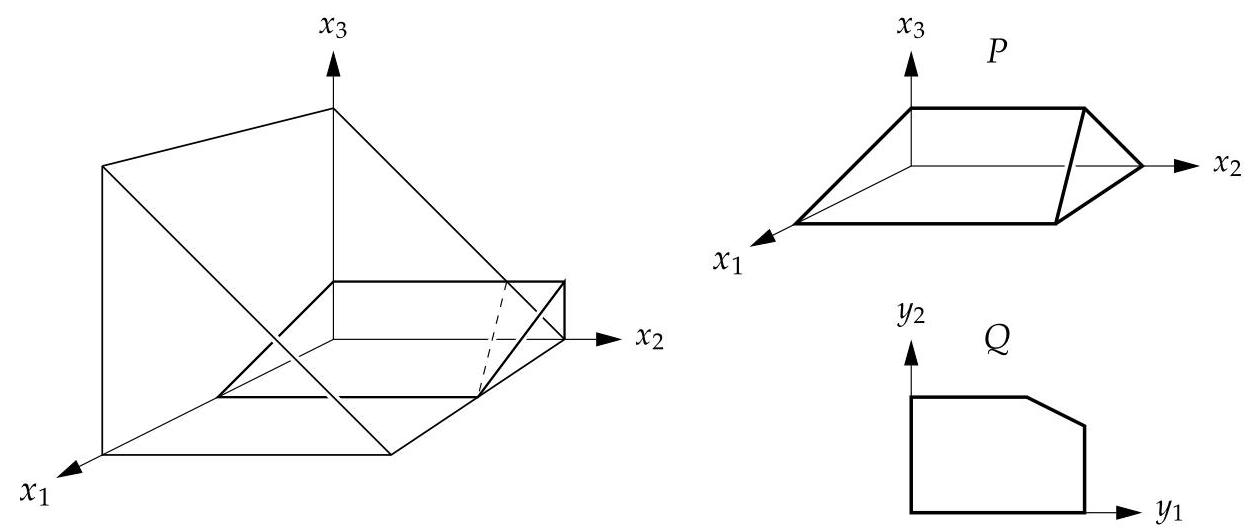
\includegraphics[max width=0.9\textwidth]{images/ch09-fig17.jpg}
\caption{示例 \eqref{eq:9.12} 中的有界多面体 \(P\) 和 \(Q\)。}
\label{fig:9.17}
\end{figure}

一般来说，我们希望 \(P\) 和 \(Q\) 是有界多面体。根据以下引理，这等价于对于任何 \(\left( {x,v}\right)  \in  \bar{P}\) 和 \(\left( {y,u}\right)  \in  \bar{Q}\) 有 \(v > 0\) 和 \(u > 0\)。


\begin{lemma} \label{lem:9.9} %引理 9.9。
考虑一个 \(m \times  n\) 双矩阵博弈 $(A, B)$。那么，式~\eqref{eq:9.24} 中的 \(P\) 是有界多面体，当且仅当对 \(X\) 中任何 \(x\) 的最优反应收益总是正的；式~\eqref{eq:9.24} 中的 \(Q\) 是有界多面体，当且仅当对 \(Y\) 中任何 \(y\) 的最优反应收益总是正的。
\end{lemma}

\begin{proof}
我们仅证明针对$Q$的情形，对 $P$ 的证明是类似的。针对任意混合策略 $y$，最优反应收益是 $Ay$ 的最大分量。因此，该收益不总是为正，当且仅当存在某个 $y \in Y$ 使得$
Ay \leq \mathbf{0}$。
对于这样的 $y$，我们有 $y \geq 0$，$y \neq \mathbf{0}$，并且对任意 $\alpha \geq 0$，都有 $y\alpha \in Q$，这表明 $Q$ 是无界的。反之，假设对任意 $y$，其最优反应收益 $u$ 始终为正。因为\(Y\) 是紧致的且 \(\bar{Q}\) 是闭集，因此\(\{ u \mid  \left( {y,u}\right)  \in  \bar{Q}\}\) 的最小值 \({u}^{\prime }\) 存在，且 \({u}^{\prime } > 0\)，并且对于 \(\bar{Q}\) 中的所有 $(y, u)$ 有 \(u \geq  {u}^{\prime }\)。此时，映射
\begin{equation}
\label{eq:9.26}
\bar{Q} \rightarrow  Q - \{ \mathbf{0}\}，\;\left( {y,u}\right)  \mapsto  y\frac{1}{u}
\end{equation}
是一个双射，其逆映射为：对于 \(z \in  Q - \{ \mathbf{0}\}\)，\(z \mapsto  \left( {z\frac{1}{{1}^{\top }z},\frac{1}{{1}^{\top }z}}\right)\)。由于 \(\frac{1}{{1}^{\top }z} \geq  {u}^{\prime }\)，因而\({\mathbf{1}}^{\top }z \leq  \frac{1}{{u}^{\prime }}\)，其中 \({\mathbf{1}}^{\top }z = \mathop{\sum }\limits_{{j = 1}}^{n}\left| {z}_{j}\right|\) 是因为 \(z \geq  \mathbf{0}\)。这证明了 \(Q\) 是有界的，从而是一个有界多面体。
\end{proof}




为了给出一个使任意$(x,v)\in \bar{P}$ 和 $(y, u)\in \bar{Q}$ 均满足 \(v > 0\) 和 \(u > 0\)的一个充分条件，我们假设
\begin{equation}\label{eq:9.27}
A ~\mbox{和 } {B}^{\top } \mbox{是非负的且没有零列}.
\end{equation}
（因为此时对于任意\(x \in  X\) 和 \(y \in  Y\)，\({B}^{\top }x\) 和 \({Ay}\) 都是非负且非零的）。我们当然可以简单地假设 \(A > 0\) 和 \(B > 0\)，但允许收益矩阵中有零元素是有用的，就像我们的示例中那样。注意，条件 \eqref{eq:9.27} 并不是最优反应收益为正的必要条件（例如，如图~\ref{fig:9.1} 所示，如果 \eqref{eq:9.1} 中 \(A\) 的左下角元素为负，最优反应收益仍然为正；另见练习~\ref{exer:9.5}）。给某个参与人的所有收益加上一个合适的正数，这不会改变该参与人的偏好（并且通过简单地减去这个常数就可以恢复原始收益），因此我们可以不失一般性地假设 \eqref{eq:9.27}。


在最优反应收益为正的情况下，有界多面体 \(P\) （除了其顶点 $\mathbf{0}$）可以通过\(\bar{P}\)得到：首先将 \(\bar{P}\) 中的每个不等式 \(\mathop{\sum }\limits_{{i = 1}}^{m}{b}_{ij}{x}_{i} \leq  v\) 除以 \(v\) 得到 \(\mathop{\sum }\limits_{{i = 1}}^{m}{b}_{ij}\left( {{x}_{i}/v}\right)  \leq  1\)，然后将 \({x}_{i}/v\) 视为一个新变量，并在 \(P\) 中仍记作\({x}_{i}\)。类似地， \(Q - \{ \mathbf{0}\}\) 是通过将 \(\bar{Q}\) 中 \({Ay} \leq  \mathbf{1}u\) 的每个不等式除以 \(u\) 得到的。实际上，我们已将期望收益归一化为 1，并去掉了条件 \({\mathbf{1}}^{\top }x = 1\) 和 \({\mathbf{1}}^{\top }y = 1\)。反过来，任意非零向量 \(x \in  P\) 和 \(y \in  Q\)，分别乘以 \(v = \frac{1}{{1}^{\top }x}\) 和 \(u = \frac{1}{{1}^{\top }y}\)，即可将它们转换为概率向量。缩放因子 \(v\) 和 \(u\) 是另一个参与人的期望收益。


\begin{figure}[htbp]
\centering
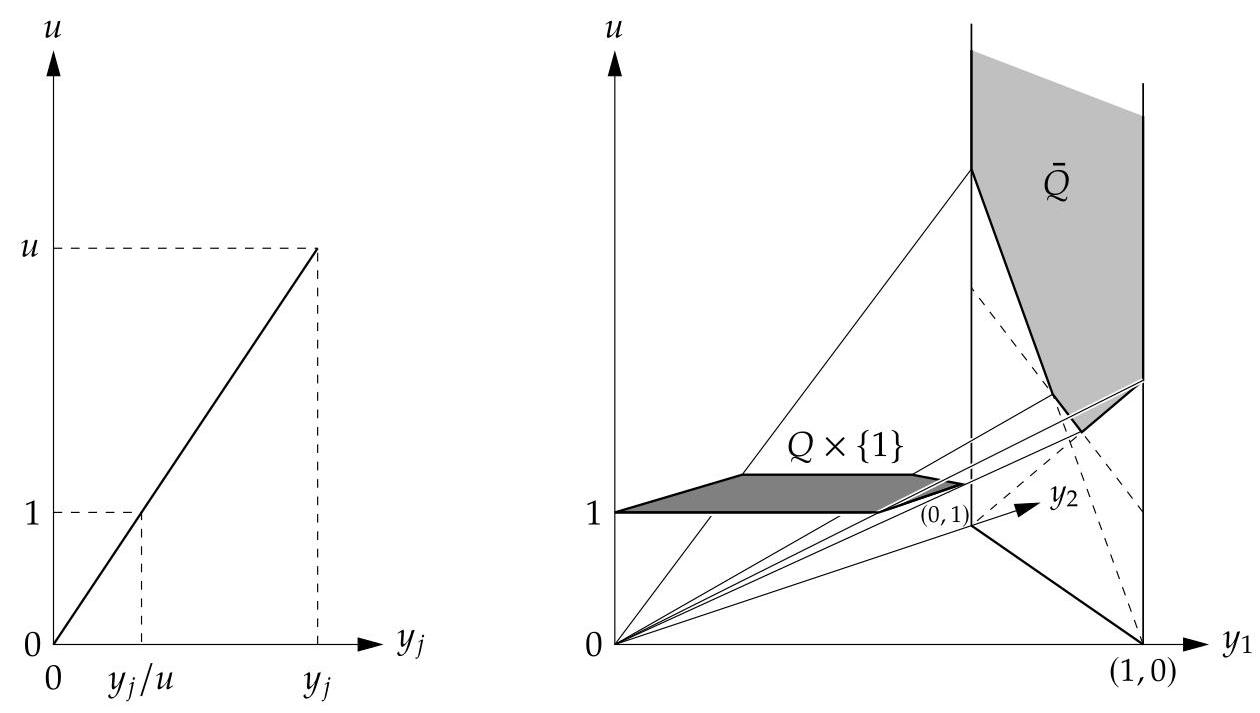
\includegraphics[max width=0.9\textwidth]{images/ch09-fig18.jpg}
\caption{式 \eqref{eq:9.26} 中的射影变换。左侧展示 \(y\) 的单个分量 \({y}_{j}\) 的情况，右侧展示如图~\ref{fig:9.1} 中的 \(\bar{Q}\) 以及式 \eqref{eq:9.25} 中的 \(Q\)。}
\label{fig:9.18}
\end{figure}

 
图~\ref{fig:9.18} 从几何角度展示了这种通过期望收益进行除法的过程，即双射\eqref{eq:9.26}，这被称为射影变换。左图展示了对于 \(y\) 的任意分量 \({y}_{j}\)，\(\left( {{y}_{j},u}\right)\) 作为 \(\bar{Q}\) 中 $(y, u)$ 的一部分。连接\(\left( {{y}_{j},u}\right)\)与 $(0,0)$ 的直线包含点 \(\left( {{y}_{j}/u,1}\right)\)。因此，\(\left( {Q-\{ \mathbf{0}\} }\right)  \times  \{ 1\}\) 是连接 \(\bar{Q}\) 中任意$(y, u)$ 与 \({\mathbb{R}}^{n} \times  \mathbb{R}\) 中 $(\mathbf{0}, 0)$ 的直线与“水平”超平面 \({\mathbb{R}}^{n} \times  \{ 1\}\) 的交点。 \(Q\) 的顶点$\mathbf{0}$并非这样的投影产生的，而是对应于 \(\bar{Q}\) 的“无穷远处”。


从 \(\bar{P}\) 到 \(P\) 的映射 \(\left( {x,v}\right)  \mapsto  x\frac{1}{v}\) 以及从 \(\bar{Q}\) 到 \(Q\) 的映射 \(\left( {y,u}\right)  \mapsto  y\frac{1}{u}\) 保持不等式关系及其紧性。因此，我们可以用参与人的纯策略 \(1,\ldots,m + n\) 对 \(P\) 和 \(Q\) 中的不等式添加标签。这也是为什么我们在式\eqref{eq:9.24}中按照 \(x \geq  \mathbf{0},{B}^{\top }x \leq  \mathbf{1}v\) 和 \({Ay} \leq  \mathbf{1}v,y \geq  \mathbf{0}\) 的顺序书写它们。由此，我们再次得到均衡的刻画：均衡对应于完全标记的点对，只不过这一次是在 \(P \times  Q - \{ \left( {\mathbf{0},\mathbf{0}}\right) \}\) 中的点对。


\begin{proposition} \label{prop:9.10} %命题9.10。
设$(A, B)$为满足式\eqref{eq:9.27}的一个双矩阵博弈，并考虑式 \eqref{eq:9.24} 定义的 \(P\) 和 \(Q\)，其中的$m+n$个不等式标记为 \(1,\ldots, m + n\)，使得任意的 \(x \in  P\) 和 \(y \in  Q\) 具有紧不等式所对应的标签。那么， \(\left( {\bar{x},\bar{y}}\right)\) 是$(A, B)$的一个均衡，且参与人I和参与人II的均衡收益分别为 \(u\) 和 \(v\)，当且仅当：\(\left( {x,y}\right)  \in  P \times  Q - \{ \left( {\mathbf{0},\mathbf{0}}\right) \}\)，且$(x, y)$是完全标记的，并满足 \(x = \bar{x}\frac{1}{v}, y = \bar{y}\frac{1}{u}, u = \frac{1}{{1}^{\top }y}\) 和 \(v = \frac{1}{{1}^{\top }x}\)。
\end{proposition}

\begin{proof}
条件 \eqref{eq:9.27} 意味着，对于任意 \(\left( {\bar{x},v}\right)  \in  \bar{P}\) 和 \(\left( {\bar{y},u}\right)  \in  \bar{Q}\)，有 \(u > 0\) 和 \(v > 0\)。因此，映射 \(\left( {\bar{x},v}\right)  \mapsto  x = \bar{x}\frac{1}{v} \in  P\) 和 \(\left( {\bar{y},u}\right)  \mapsto  y = \bar{y}\frac{1}{u} \in  Q\) 是定义{\color{red}完备}的，并且它们保持不等式关系以及这些不等式取紧等号的情形。这表明，\(\bar{x}\) 的标签就是 \(x\) 的标签，\(\bar{y}\) 的标签就是 \(y\) 的标签。由此，如果 \(\left( {\bar{x},\bar{y}}\right)\) 是一个均衡，那么根据推论 \ref{coro:9.8}可知，\(\left( {\bar{x},\bar{y}}\right)\) 是完全标记的，从而$(x, y)$也是完全标记的。


反之，假设 \(\left( {x,y}\right)  \in  P \times  Q\) 是完全标记的，且 \(\left( {x,y}\right)  \neq  \left( {\mathbf{0},\mathbf{0}}\right)\)。如果 \(x = \mathbf{0}\)，那么必然有\(y \neq  \mathbf{0}\)。因此，存在某个 \(j \in  \{ 1,\ldots,n\}\) 使得\({y}_{j} \neq  0\)，从而\(y\) 没有标签 \(m + j\)。这意味着$(x, y)$不是完全标记的，因为 \(x\) 只有标签 \(1,\ldots,m\)，产生矛盾。因此，\(x \neq  \mathbf{0}\)。类似地，\(y \neq  \mathbf{0}\)。通过同样的推理，\(x\) 必然有某个标签 \(m + j\)。根据式 \eqref{eq:9.23}，这意味着 \({B}^{\top }x \leq  \mathbf{1}\) 中至少有一个不等式是紧的。因此，\(v = \frac{1}{{1}^{\top }x}\) 是 \(\left( {\bar{x},v}\right)  \in  \bar{P}\) 针对 \(\bar{x} = {xv}\) 的最优反应收益。类似地，\(P\) 中的 \(y\) 有某个标签 \(i \in  \{ 1,\ldots,m\}\)，这意味着 \({\left( Ay\right) }_{i} = 1\)。因此，\(u = \frac{1}{{1}^{\mathrm{\;T}}y}\) 是 \(\left( {\bar{y},u}\right)  \in  \bar{Q}\) 针对 \(\bar{y} = {yu}\) 的最优反应收益。
\end{proof}


上述证明的最后一段表明，当考虑 \(P \times  Q\) 中完全标记的点对 $(x, y)$ 时，我们无需担心 \(P\) 或 \(Q\) 中出现 \({B}^{\top }x < \mathbf{1}\) 或 \({Ay} < \mathbf{1}\) 的情况（即不存在紧不等式）。有一个明显的例外，即 \(P \times  Q\) 中的点对 $(\mathbf{0},\mathbf{0})$，它自然地充当了莱姆基 - 豪森算法的人工均衡点；与\(\widetilde{X} \times  \widetilde{Y}\) 的情形不同，这里无需额外添加该点。对于示例\eqref{eq:9.1}，图~\ref{fig:9.19} 展示了 \(P \times  Q\) 上缺失标签 2 的莱姆基 - 豪森路径。它们遍历了 \(P\) 和 \(Q\) 中几乎完全标记的顶点对，我们通过它们的标签集来精确识别这些顶点对，就像在式\eqref{eq:9.7} 和 \eqref{eq:9.8} 中那样。


\begin{figure}[htbp]
\centering
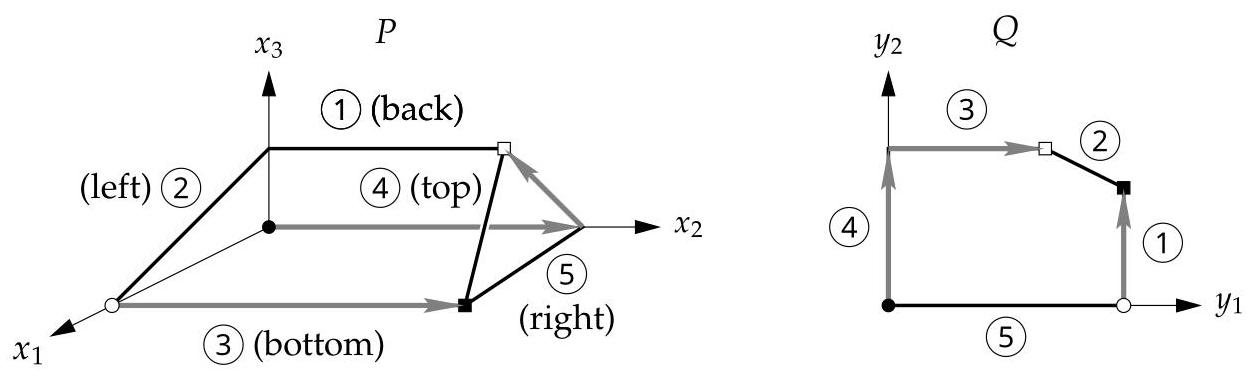
\includegraphics[max width=0.9\textwidth]{images/ch09-fig19.jpg}
\caption{图~\ref{fig:9.5} 中在多面体 \(P\) 和 \(Q\) 上缺失标签 2 的莱姆基-豪森路径。}
\label{fig:9.19}
\end{figure}


\section{互补换基法} \label{sec9.7}


本节从代数角度描述莱姆基 - 豪森算法在任意维度下的工作原理。我们先考虑一个 \(m \times  n\) 双矩阵博弈 $(A, B)$。设 \(C\) 是如下定义的 \(d \times  d\) 矩阵：
\begin{equation}
\label{eq:9.28}
d = m + n,\;\;C = \left( \begin{matrix} 0 & A \\  {B}^{\top } & 0 \end{matrix}\right) .
\end{equation}



与式 \eqref{eq:9.27} 一致，不失一般性，我们假设 \(C\) 是非负的且没有零列。那么，\(S = P \times  Q\) 是一个有界多面体，并可以写成
\begin{equation}
\label{eq:9.29}
S = \left\{  {z \in  {\mathbb{R}}^{d} \mid  z \geq  \mathbf{0}, ~~ {Cz} \leq  \mathbf{1}}\right\},
\end{equation}
其中 \(z \in  S = P \times  Q\) 表示
\begin{equation}
\label{eq:9.30}
z = \left( {x,y}\right)，\;{z}_{i} = {x}_{i}\;\left( {1 \leq  i \leq  m}\right)，\;{z}_{m + j} = {y}_{j}\;\left( {1 \leq  j \leq  n}\right).
\end{equation}


我们用标签 \(1,\ldots,d\) 标记式\eqref{eq:9.29} 中的 \(d\) 个不等式 \(z \geq  \mathbf{0}\) 和 \(d\) 个不等式 \({Cz} \leq  \mathbf{1}\)。这\(d\) 个标签按照式\eqref{eq:9.2} 和 \eqref{eq:9.23} 的方式对应于参与人的纯策略。与前文一样，\(S\) 中的任意点\(z\)获得那些紧不等式对应的标签。通过命题 \ref{prop:9.10}中所示的归一化 \(\bar{x} = x\frac{1}{{\mathbf{1}}^{\top }x}\) 和 \(\bar{y} = y\frac{1}{{\mathbf{1}}^{\top }y}\) 可以得到，博弈$(A, B)$ 的一个均衡 \(\left( {\bar{x},\bar{y}}\right)\) 对应于 \(S - \{ \mathbf{0}\}\) 的一个完全标记点 \(z = \left( {x,y}\right)\)，即 \(z\) 拥有所有标签 \(1,\ldots,d\)。

为了进行代数处理，我们用非负的松弛变量\(w \in  {\mathbb{R}}^{d}\) 将式 \eqref{eq:9.29} 中的不等式 \({Cz} \leq  \mathbf{1}\) 写成等式\({Cz} + w = \mathbf{1}\)和非负性约束 \(w \geq  \mathbf{0}\)。于是，\(z \in  S\) 具有标签 \(i \in  \{ 1,\ldots,d\}\) 当且仅当 \({z}_{i} = 0\) 或 \({w}_{i} = 0\)，即 \({z}_{i}{w}_{i} = 0\)。如果对于所有的 \(i = 1,\ldots,d\) 都有\({z}_{i}{w}_{i} = 0\)，那么称向量 \(z\) 和 \(w\) 是互补的。由此，在 \(S\) 中找到一个完全标记点 \(z\) 的问题，可以转变为：在 \({\mathbb{R}}^{d}\) 中找到 \(z\) 和 \(w\)，使得
\begin{equation}
\label{eq:9.31}
{Cz} + w = \mathbf{1},\;z \geq  \mathbf{0},\;w \geq  \mathbf{0},\;{z}_{i}{w}_{i} = 0\;\left( {1 \leq  i \leq  d}\right).
\end{equation}


做个总结：如果 \(z \in  S\)，并定义 \(w = \mathbf{1} - {Cz}\)，那么有 \(z \geq  \mathbf{0}\) 和 \(w \geq  \mathbf{0}\)，并且 \(z\) 是完全标记的当且仅当 \(z\) 和 \(w\) 是互补的。

回顾一下，如果 \({z}_{i} = 0\) 或 \({w}_{i} = 0\)，则 \(z\) 有标签 \(i\)。因此，缺失标签意味着存在某个 \(\ell  \in  \{ 1,\ldots,d\}\)，使得 \({z}_{\ell } > 0\) 和 \({w}_{\ell } > 0\)成立。如果除了这个例外，式\eqref{eq:9.31} 中的所有其他条件都成立，那么 \(z\) 和 \(w\) 被称为几乎互补。这意味着 \(z\) 是 \(S\) 中的一个几乎完全标记的点，即 \(z\) 具有除可能的\(\ell\)之外的所有标签。


莱姆基 - 豪森算法从式 \eqref{eq:9.31}  的平凡解 \(z = \mathbf{0},w = \mathbf{1}\) 开始，该解即为人工均衡。对于例子\eqref{eq:9.1}，系统 \(w = 1 - {Cz}\) 表述为
\begin{equation}
\label{eq:9.32}
\begin{aligned}
{w}_{1} & = 1\; - 2{z}_{4} \\
{w}_{2} & = 1\; - \;{z}_{4} - 2{z}_{5} \\
{w}_{3} & = 1\; - 3{z}_{5} \\
{w}_{4} & = 1\; - 2{z}_{1}\; - 4{z}_{3}  \\
{w}_{5} & = 1\; - {z}_{2} - {z}_{3}.
\end{aligned}
\end{equation}

这被称为一个字典，其含义是某些变量（这里是 \(w_{1},\ldots,w_{5}\)）被表示为其他变量（这里是 \(z_{1},\ldots,z_{5}\)）的函数。左侧的因变量称为基变量，右侧的自变量称为非基变量。通过将所有非基变量设为零来得到相应的基解，此时所有基变量等于字典中的常数项。如果这些常数都是非负的，那么该基解被称为可行解。式\eqref{eq:9.32}的基解是 \(z = \mathbf{0},w = \mathbf{1}\)，即为可行解。


莱姆基 - 豪森算法通过换基操作进行迭代。该操作以这样一种方式交换一个非基变量和一个基变量：新的字典仍然定义变量之间相同的线性关系，并且相应的基解仍然保持可行。从几何角度来看，每个基本可行解定义了有界多面体 \(S\) 的一个顶点，换基操作意味着沿着 \(S\) 的一条边，从一个顶点移动到相邻的顶点，如图~\ref{fig:9.19} 所示。我们将进行说明。


选择一个固定的缺失标签 \(\ell  \in  \{ 1,\ldots, d\}\)，这里取 \(\ell  = 2\)，它确定了入基变量 \({z}_{\ell }\)。在当前的基解中，所有非基变量都被设为零，但现在入基变量（在 式\eqref{eq:9.32}  中是 \({z}_{2}\)）被允许取正值。字典 \eqref{eq:9.32} 描述了这如何改变左边的基变量，这里只有变量 \({w}_{5}\)，因为 \({z}_{2}\) 只出现在最后一个方程 \({w}_{5} = 1 - {z}_{2} - {z}_{3}\)。约束 \({w}_{5} \geq  0\) 限制了 \({z}_{2}\) 的增加，因为当 \({z}_{2} = 1\) 时 \({w}_{5}\) 变为零。这就确定了 \({w}_{5}\) 为离基变量。



接下来的换基步骤是让 \({z}_{2}\) 进入基 且 \({w}_{5}\) 离开基，这意味着重写字典使得 \({z}_{2}\) 变为基变量且\({w}_{5}\) 变为非基变量。此时，简单地将 \({w}_{5}\) 与 \({z}_{2}\) 交换即可定义新的字典
\begin{equation}
\label{eq:9.33}
\begin{aligned}
{w}_{1} & = 1\; - 2{z}_{4} \\
{w}_{2} & = 1\; - \;{z}_{4} - 2{z}_{5} \\
{w}_{3} & = 1\; - 3{z}_{5} \\
{w}_{4} & = 1\; - 2{z}_{1}\; - 4{z}_{3}  \\
{z}_{2}  & = 1\; - {w}_{5} - {z}_{3}.
\end{aligned}
\end{equation}


在这个新字典的基解中，\({z}_{2} = 1\) 和 \({w}_{5} = 0\)。在图~\ref{fig:9.19}中，这是 \(P\) 中从顶点 \(x = \left( {0,1,0}\right)\) 出发的第一个箭头的终点，其中标签2被去掉，标签5被选取（因为 \({w}_{5}\) 已变为非基变量）。在 \(Q\) 中，我们仍然有 \(\left( {{y}_{1},{y}_{2}}\right)  = \left( {{z}_{4},{z}_{5}}\right)  = \left( {0,0}\right)\)。


字典\eqref{eq:9.33} 有两个非基变量 \({z}_{5}\) 和 \({w}_{5}\)，它们的下标都是5，这就是重复标签。根据互补换基法规则，因为 \({w}_{5}\) 刚刚离开基，所以它的互补变量 \({z}_{5}\) 被选为下一个入基变量。


也就是说，从与 \eqref{eq:9.33} 相关的基解开始，允许 \({z}_{5}\) 变为正数，而所有其他非基变量保持为零。仅考虑 \({z}_{5}\) 的增加，等式左边受影响的变量是 \({w}_{2} = 1 - 2{z}_{5}\) 和 \({w}_{3} = 1 - 3{z}_{5}\)，它们都应保持非负。这些约束中更强的是 \({w}_{3} = 1 - 3{z}_{5} \geq  0\)；因为，当 \({z}_{5} = \frac{1}{3}\) 时， \({w}_{3}\) 变为零，而 \({w}_{2}\) 仍然为正。因此， \({w}_{3}\) 是离基变量。换基操作步骤现在意味着将第三个方程（目前左边是 \({w}_{3}\)）重写为 \({z}_{5} = \frac{1}{3} - \frac{1}{3}{w}_{3}\)，并将这个表达式代入 \({z}_{5}\) 在右边其他地方出现的位置。唯一的代入是这里的 \({w}_{2} = 1 - {z}_{4} - 2{z}_{5} = 1 - {z}_{4} - 2\left( {\frac{1}{3} - \frac{1}{3}{w}_{3}}\right)\)。所以，得到的新字典是
\begin{equation}
\label{eq:9.34}
\begin{aligned}
{w}_{1} & = 1\; - 2{z}_{4} \\
{w}_{2} & = \frac{1}{3}\; - \;{z}_{4} + \frac{2}{3}{w}_{3}\\
{z}_{5} & = \frac{1}{3}\; - \frac{1}{3}{w}_{3}\\
{w}_{4} & = 1\; - 2{z}_{1}\; - 4{z}_{3}  \\
{z}_{2}  & = 1\; - {w}_{5} - {z}_{3}.
\end{aligned}
\end{equation}


在前面的换基操作步骤中，\({z}_{5}\) 入基， \({w}_{3}\) 离基。在图~\ref{fig:9.19}中，在 \(Q\) 中去掉了标签5，选取了标签3，新的基解位于 \(Q\) 的顶点 \(y = \left( {0,\frac{1}{3}}\right)\) 处。

根据互补换基法规则，式\eqref{eq:9.34}中的下一个入基变量是 \({z}_{3}\)，它是 \({w}_{3}\) 的互补变量。 \({z}_{3}\) 的增加产生了两个约束 \({w}_{4} = 1 - 4{z}_{3} \geq  0\) 和 \({z}_{2} = 1 - {z}_{3} \geq  0\)，其中前者更强，因为当 \({z}_{4} = \frac{1}{4}\) 时 \({w}_{4}\) 变为零。因此，离基变量是 \({w}_{4}\)，所以我们将第四个方程重写为 \({z}_{3} = \frac{1}{4} - \frac{1}{2}{z}_{1} - \frac{1}{4}{w}_{4}\)，并将其代入含有 \({z}_{3}\) 的表达式：
\begin{equation}
\label{eq:9.35}
\begin{aligned}
{w}_{1} & = 1\; - 2{z}_{4} \\
{w}_{2} & = \frac{1}{3}\; - \;{z}_{4} + \frac{2}{3}{w}_{3}\\
{z}_{5} & = \frac{1}{3}\; - \frac{1}{3}{w}_{3}\\
{z}_{3} & = \frac{1}{4} - \frac{1}{2}{z}_{1}\; - \frac{1}{4}{w}_{4}  \\
{z}_{2} & = \frac{3}{4} + \frac{1}{2}{z}_{1} - {w}_{5} + \frac{1}{4}{w}_{4}.
\end{aligned}
\end{equation}


在前面的换基操作步骤中，\({z}_{3}\) 入基， \({w}_{4}\) 离基。这意味着在 \(P\) 中，去掉了标签3，选取了标签4，并且 \(x\) 移动到 \(P\) 的新顶点 \(\left( {0,\frac{3}{4},\frac{1}{4}}\right)\)，这已经是图~\ref{fig:9.19}中 \(P\) 里的白色方块。

作为已离基的 \({w}_{4}\) 的互补变量，式\eqref{eq:9.35}中的新入基变量是 \({z}_{4}\)。在两个约束条件 \({w}_{1} = 1 - 2{z}_{4} \geq  0\) 和 \({w}_{2} = \frac{1}{3} - {z}_{4} \geq  0\) 中，第二个更强，因为当 \({z}_{4} = \frac{1}{3}\) 时 \({w}_{2}\) 变为零。我们将第二个方程重写为 \({z}_{4} = \frac{1}{3} - {w}_{2} + \frac{2}{3}{w}_{3}\)，并将其代入含有 \({z}_{4}\) 的表达式：
\begin{equation}
\label{eq:9.36}
\begin{aligned}
{w}_{1} & = \frac{1}{3}\; + 2{w}_{2} - \frac{4}{3}{w}_{3}  \\
{z}_{4} & = \frac{1}{3}\; - \;{w}_{2} + \frac{2}{3}{w}_{3}  \\
{z}_{5} & = \frac{1}{3}\; - \frac{1}{3}{w}_{3}  \\
{z}_{3} & = \frac{1}{4} - \frac{1}{2}{z}_{1}\; - \frac{1}{4}{w}_{4} \\
{z}_{2} & = \frac{3}{4} + \frac{1}{2}{z}_{1} - {w}_{5} + \frac{1}{4}{w}_{4}.
\end{aligned}
\end{equation}

因为 \({z}_{4}\) 入基且 \({w}_{2}\) 离基，这意味着在 \(Q\) 中标签 4 被去掉，标签 2 被选取，\(Q\) 的新顶点为 \(y = \left( {\frac{1}{3},\frac{1}{3}}\right)\)，即图~\ref{fig:9.19} 中 \(Q\) 里的白色方块。


算法终止。因为离基变量的下标是缺失标签 \(\ell  = 2\)，所以现在该下标对应的基变量只有一个，而不像所有中间步骤中那样存在两个。与最终字典\eqref{eq:9.36}对应的基解满足方程组 \eqref{eq:9.31}。这个解是 \(z = \left( {x,y}\right)\)，其中 \(x = \left( {0,\frac{3}{4},\frac{1}{4}}\right)\) 和 \(y = \left( {\frac{1}{3},\frac{1}{3}}\right)\)。它定义了一个均衡 \(\left( {\bar{x},\bar{y}}\right)\)，其中 \(\bar{x} = x\)，参与人 II 的收益为 1，以及 \(\bar{y} = \left( {\frac{1}{2},\frac{1}{2}}\right)\)，参与人 I 的收益为 \(\frac{3}{2}\)。


在本节的其余部分，我们将一般性地描述互补换基法。目前，我们假设式 \eqref{eq:9.29} 中的有界多面体 \(S\) 是非退化的，这意味着 \(S\) 中没有点的紧不等式超过 \(d\) 个。这也等价于博弈 $(A, B)$ 是非退化的。


借助 \(d \times  d\) 单位矩阵 \(I\)，我们将式 \eqref{eq:9.31}  中的方程组写为 \({Cz} + {Iw} = \mathbf{1}\)。这个系统的变量是 \(z\) 和 \(w\) 的 \({2d}\) 个分量，系数矩阵是 \(\left\lbrack  {CI}\right\rbrack\)，右侧常数是$ \mathbf{1}$。矩阵 \(\left\lbrack  {CI}\right\rbrack\) 中任意 \(d\) 个线性无关的列定义了一个可逆矩阵 \(D\)，称为基矩阵。与这些基列相对应的变量 \({z}_{i}\) 或 \({w}_{i}\) 称为基变量；其他列和变量分别称为非基列和非基变量。

用基矩阵 \(D\) 的逆矩阵乘以系统 \({Cz} + {Iw} = \mathbf{1}\)，得到等价的系统
\begin{equation}
\label{eq:9.37}
{D}^{-1}{Cz} + {D}^{-1}w = {D}^{-1}\mathbf{1}.
\end{equation}

这个新系统与上述 \eqref{eq:9.32}  - \eqref{eq:9.36} 中的字典形式类似，只是我们将基变量和非基变量都保留在了等式的左侧。原因是在系统 \eqref{eq:9.37} 中，基变量的列定义了单位矩阵，所以 \eqref{eq:9.37} 展示了基变量如何依赖于非基变量。当非基变量设为零时，基变量等于 \({D}^{-1}\mathbf{1}\)，这（连同为零的非基变量）定义了对应于系统\eqref{eq:9.37} 的基解。如果这个基解 \(z,w\) 是非负的，即 \({D}^{-1}\mathbf{1} \geq  \mathbf{0}\)，则称其为可行解。根据非退化性，这意味着 \({D}^{-1}\mathbf{1} > \mathbf{0}\)，即所有基变量都取正值。


换基操作意味着选择一个非基变量进入基，同时选择一个基变量离开基。假设入基变量是 \({z}_{j}\)（若以某个 \({w}_{j}\) 作为入基变量，过程完全相同）。假设当前的基解是可行的，并且希望在\({z}_{j}\) 从零开始增大时仍保持解的可行性。 \({z}_{j}\) 的增大改变了那些当前值等于向量 \({D}^{-1}\mathbf{1}\) 的基变量，我们用 \(q\) 表示这些基变量。假设向量 \(v\) 是  \eqref{eq:9.37}  中对应于 \({z}_{j}\) 的非基列。随着 \({z}_{j}\) 的增大，基变量组成的向量由 \(q - v{z}_{j}\) 给出，并且应该保持非负，这意味着对于所有行 \(i = 1,\ldots,d\) 都有 \({q}_{i} - {v}_{i}{z}_{j} \geq  0\)。因为 \(q \geq  \mathbf{0}\) 已经成立，所以我们只需要考虑满足 \({v}_{i} > 0\) 的行 \(i\)。如果 \(v\) 没有正元素，我们可以无限增大 \({z}_{j}\)，这将在 \(S\) 中定义一条无界的“射线”，但 \(S\) 是有界的，所以这种情况不会发生（互补换基法也适用于一般矩阵 \(C\)，此时算法可能会出现“射线终止”的情况）。


因此，入基列 \(v\) 至少有一个正分量 \({v}_{i}\)，且\({z}_{j}\) 的增大受到条件 \(q - v{z}_{j} \geq  \mathbf{0}\) 的限制，即对于所有满足 \({v}_{i} > 0\) 的 \(i\) 都有 \({q}_{i} \geq  {v}_{i}{z}_{j}\)，或者等价地
\begin{equation}
\label{eq:9.38}
{z}_{j} \leq  \min \left\{  {\frac{{q}_{i}}{{v}_{i}} \mid  i = 1,\ldots,d,\; {v}_{i} > 0}\right\}.
\end{equation}

当 \({z}_{j}\) 恰好等于式\eqref{eq:9.38} 中的最小值时，不等式 \({q}_{i} - {v}_{i}{z}_{j} \geq  0\) 中有一个取等号。这样的行 \(i\) 确定了离基变量。求解式 \eqref{eq:9.38}中的最小值也称为最小比值检验。

非退化性意味着式 \eqref{eq:9.38} 中的最小值以及离基变量是唯一的。原因是，如果最小值在两行（或更多行）中取得，那么在对应的两个基变量中只能选择一个离开基，而另一个将保持为基变量，并且在换基步骤之后其值将为零，这意味着新的基是退化的。我们将在下一节给出一个这样的例子。

系统 \eqref{eq:9.37} 中入基变量 \({z}_{j}\) 所在的列以及离基变量所在的行，共同确定了主元 \({v}_{i}\)。根据式\eqref{eq:9.38} 可知，主元是正的。换基操作用入基变量替换离基变量，这意味着用入基变量对应的列替换基矩阵\(D\)中离基变量对应的列。不必从头计算新基矩阵的逆 \({D}^{-1}\)，只需对系统 \eqref{eq:9.37} 进行行变换，将入基列变为单位向量 \({e}_{i}\) 即可。在这些行变换中，主元行除以主元 \({v}_{i}\)，并从其他行中减去主元行的适当倍数。正如上面的例子 \eqref{eq:9.32}  - \eqref{eq:9.35}，这些行变换体现为从一个字典到下一个字典的代数替换。


如前所述，换基操作是一种沿着多面体的边从一个顶点移动到另一个顶点的一般方法，其中每个顶点对应一个基本可行解。在线性规划中，即在多面体上最大化一个线性函数的问题，换基操作是非常重要的单纯形算法的主要操作。

互补换基法的特殊之处在于其初始化和下一个入基变量的选择，其目标是求解系统 \eqref{eq:9.31}，即找到一个互补解 \(z,w\)。一个初始互补解是 \(z = \mathbf{0}\) 和 \(w = \mathbf{1}\)。通过放宽互补性条件，允许一个下标 \(\ell\)（对应缺失标签），使得 \({z}_{\ell }\) 和 \({w}_{\ell }\) 都可以取正值，从而二者都可以成为基变量，以此来提供沿着路径移动的自由度。

在初始互补解 \(z = \mathbf{0}\) 和 \(w = \mathbf{1}\) 处，第一个入基变量是 \({z}_{\ell }\)。一旦 \({z}_{\ell }\) 进入基，变量 \({w}_{i}\) 就变成了非基变量，此时它与 \({z}_{i}\) 一起成为非基变量。互补换基规则是：将离基变量的互补变量作为下一个入基变量。\({w}_{i}\) 的互补变量是 \({z}_{i}\)，反之亦然（同一个变量可能多次进入和离开基，因此也有可能某个 \({z}_{i}\) 离开基，随后 \({w}_{i}\) 又进入基）。缺失标签 \(\ell\) 为算法提供了唯一的起始点，随后唯一的离基变量和互补换基规则意味着每一步都有唯一的延续。因此，算法以唯一的方式进行，并且不会重新访问几乎互补的基。当 \({w}_{\ell }\) 或 \({z}_{\ell }\) 离开基时，算法终止，然后得到系统 \eqref{eq:9.31} 的解。


从几何角度看，这描述了有界多面体 \(S\) 的一条边路径。该路径上的点具有集合\(\{ 1,\ldots,d\}  - \{ \ell \}\) 中的所有标签，并且路径的端点是完全标记的。对于 式\eqref{eq:9.28}  中的 \(C\)，这就是在 \(S = P \times  Q\) 上缺失标签 \(\ell\) 的莱姆基 - 豪森路径，正如图~\ref{fig:9.19} 所示的那样。


\section{退化博弈的求解}    \label{sec9.8}

当博弈是退化的且离基变量并不总是唯一时，我们可以利用一种扩展的莱姆基 - 豪森算法进行求解均衡。作为示例，考虑例\eqref{eq:9.1}的一个变形：
\begin{equation}
\label{eq:9.39}
A = \left( \begin{array}{ll} 2 & 0 \\  1 & 2 \\  0 & 3 \end{array}\right), \;\;B = \left( \begin{array}{ll} 2 & 0 \\  1 & 1 \\  4 & 1 \end{array}\right),
\end{equation}
其中 \(B\) 的两列都是针对第二行的最优反应，因此该博弈是退化的。那么，初始字典 \eqref{eq:9.32}的最后两行需要改为
\begin{equation}
\label{eq:9.40}
\begin{aligned}
{w}_{4} & = 1 - 2{z}_{1} - {z}_{2} - 4{z}_{3} \\
{w}_{5} & = 1\; - {z}_{2} - {z}_{3}.
\end{aligned}
\end{equation}

对于缺失标签 \(\ell  = 2\)，选择第一个入基变量 \({z}_{2}\)。当 \({z}_{2} = 1\) 时，\({w}_{4}\) 和 \({w}_{5}\) 同时变为零。跟之前一样，我们选择 \({w}_{5}\) 作为离基变量。那么，式\eqref{eq:9.40} 可以重写为
\begin{equation}
\label{eq:9.41}
\begin{aligned}
{w}_{4} & = 0 - 2{z}_{1} + {w}_{5} - 3{z}_{3} \\
{z}_{2} & = 1\; - {w}_{5} - {z}_{3},
\end{aligned}
\end{equation}
这将替换 \eqref{eq:9.33} 中的最后两行。下一个入基变量是 \({z}_{5}\)，离基变量是 \({w}_{3}\)，并由此得到字典\eqref{eq:9.34}，但其最后两行用 \eqref{eq:9.41} 替换。下一个入基变量是\eqref{eq:9.41} 中的 \({z}_{3}\)，而离基变量必然是 \({w}_{4}\)，因为在保持 \({w}_{4}\) 非负的情况下，\({z}_{3}\) 根本无法增加。于是，从 \eqref{eq:9.41} 得到的新（部分）字典是
\begin{equation}
\label{eq:9.42}
\begin{aligned}
{z}_{3} & = 0 - \frac{2}{3}{z}_{1} + \frac{1}{3}{w}_{5} - \frac{1}{3}{w}_{4} \\
{z}_{2} & = 1 + \frac{2}{3}{z}_{1} - \frac{4}{3}{w}_{5} + \frac{1}{3}{w}_{4},
\end{aligned}
\end{equation}
它与字典 \eqref{eq:9.41} 有相同的基本可行解，其中 \({z}_{3} = 0\) 和 \({w}_{4} = 0\)。因此，它们对应于 \(P\) 中的同一个顶点 $(0, 1, 0)$，只是基发生了变化。具体而言，唯一的区别是：在 \eqref{eq:9.41} 中 \({w}_{4}\) 是基变量，\({z}_{3}\) 是非基变量，而在 \eqref{eq:9.42} 中则相反。

此时，新的字典由方程组 \eqref{eq:9.42} 替换\eqref{eq:9.35} 中的最后两行，其中新的入基变量是 \({z}_{4}\)，它是离开基的变量 \(w_{4}\) 的互补变量。这个字典仍然得到与\eqref{eq:9.35} 中相同的最终换基操作步骤，即 \({w}_{2}\) 离基；最终的字典由 \eqref{eq:9.36} 的前三行和\eqref{eq:9.42}中的两个方程组成。由此得到博弈\eqref{eq:9.39} 的均衡 \(\left( {\bar{x},\bar{y}}\right)\) 为 \(\bar{x} = \left( {0,1,0}\right)\) 和 \(\bar{y} = \left( {\frac{1}{2},\frac{1}{2}}\right)\)。

在本例中，该算法仍然成功找到了博弈的一个均衡。然而，我们不再能保证它在一般情况下会终止。由于存在多个可能的离基变量，类似于图\ref{fig:9.6}中的城堡现在有多于两扇门的房间，因此完全可能通过第三扇门重新进入这样的房间，从而导致无限循环。


当存在退化基（即基本可行解中某些基变量的取值为零）时，就会出现这个问题。解决这个问题的方法是，通过对系统 \({Cz} + {Iw} = \mathbf{1}\) 的右侧$\mathbf{1}$进行微扰，确保基本可行解中的基变量始终为正。微扰可以是任意小（趋近于零），因此实际上是虚构的，它只是为离基变量引入了某种确定性规则。

考虑一个新参数 \(\varepsilon  > 0\)，它将被设为任意小。修改后的系统为 \({Cz} + {Iw} = \mathbf{1} + {\left( \varepsilon,{\varepsilon }^{2},\ldots,{\varepsilon }^{d}\right) }^{\top }\)，因此对于基矩阵 \(D\) 的系统 \eqref{eq:9.37} 变为
\begin{equation}
\label{eq:9.43}
{D}^{-1}{Cz} + {D}^{-1}w = {D}^{-1}\mathbf{1} + {D}^{-1}{\left( \varepsilon，{\varepsilon }^{2},\ldots,{\varepsilon }^{d}\right) }^{\top }.
\end{equation}

如果 \(\varepsilon  = 0\)，这就是原始系统\eqref{eq:9.37}，此时若 \({D}^{-1}\mathbf{1} \geq 0\)，则对应的基解是可行的。我们现在希望加强这一条件，使得当 \(\varepsilon\) 取足够小的正值时，基解仍然为正值。当 \({D}^{-1}\mathbf{1} > 0\) 时，这显然成立；但对于退化基，这个向量可能有零分量。用 \({r}_{i} = \left( {{q}_{i0},{q}_{i1},\ldots,{q}_{id}}\right)\) 表示拼接矩阵 \(\left\lbrack  {{D}^{-1}\mathbf{1}~~{D}^{-1}}\right\rbrack\) 的第 \(i\) 行。那么，当\(\varepsilon\)取足够小的正值时，系统\eqref{eq:9.43} 的右端全为正，当且仅当对所有 \(i = 1,\ldots,d\)，\({r}_{i}\) 的第一个非零元素为正。这是因为 \eqref{eq:9.43}的第 \(i\) 行是 \({q}_{i0} + {q}_{i1}\varepsilon  + {q}_{i1}{\varepsilon }^{2} + \cdots  + {q}_{id}{\varepsilon }^{d}\)，并且在 \(\varepsilon\) 足够小时，第一个非零求和项（比如 \({q}_{ij}{\varepsilon }^{j}\)）会大于所有包含 \(\varepsilon\) 更高次幂的其余求和项。注意，\({r}_{i}\) 不可能是全零行向量，因为它的最后 \(d\) 个分量是 \({D}^{-1}\) 的一行，而\({D}^{-1}\)是可逆矩阵。如果矩阵 
\(\left\lbrack  {{D}^{-1}\mathbf{1}~~{D}^{-1}}\right\rbrack\) 的每一行 \({r}_{i}\) 的第一个非零分量均为正，则称该矩阵为字典正序。显然，当初始基变量为 \(w\) 且 \(D = I\) 时，该条件成立，并且算法将在后续步骤中保持这一条件。这意味着，对于足够小的正值 \(\varepsilon\)，扰动后的系统\eqref{eq:9.43} 永远不会出现退化情况。


因此，在换基操作的每一步中，离基变量总是唯一的，并且可以通过如下所示的最小比值检验 \eqref{eq:9.38} 的推广形式确定。假设入基变量是 \({z}_{j}\) （类似地，也可以是 \({w}_{j}\)），其入基列是 \(v\)，该列至少有一个正分量 \({v}_{i}\)。在扰动系统 \eqref{eq:9.43}中，增加入基变量\({z}_{j}\)时，需满足的约束条件是：对于所有满足 \({v}_{i} > 0\) 的行 \(i\)，
\begin{equation}
\label{eq:9.44}
{z}_{j} \leq  \frac{{q}_{i0}}{{v}_{i}} + \frac{{q}_{i1}}{{v}_{i}}\varepsilon  + \frac{{q}_{i2}}{{v}_{i}}{\varepsilon }^{2} + \cdots  + \frac{{q}_{id}}{{v}_{i}}{\varepsilon }^{d}.
\end{equation}

式 \eqref{eq:9.44} 中 \(1,\varepsilon,{\varepsilon }^{2},\ldots,{\varepsilon }^{d}\) 的系数由行向量 \(\frac{1}{{v}_{i}}{r}_{i}\) 给出。我们考虑这些行向量按字典序最小的那个，即，在这些分量不同的情况下，第一个分量最小的那个。例如，在如下的行向量中，
\[
\left( {0,0,2, - 1}\right),\;\left( {0,0,1,{1000}}\right),\;\left( {0,3, - {100}, - 8}\right),
\]
第二行是按字典序最小的。按字典序最小的行是唯一的，因为如果两行相同，比如 \(\frac{1}{{v}_{i}}{r}_{i}\) 和 \(\frac{1}{{v}_{k}}{r}_{k}\)，则\({D}^{-1}\) 有两个线性相关的行，这与\({D}^{-1}\)可逆相矛盾。在式 \eqref{eq:9.44} 中选择按字典序最小的行 \(\frac{1}{{v}_{i}}{r}_{i}\) 称为字典序最小比率检验。因为这一行是字典正序的，所以 \({z}_{j}\) 在扰动系统中进入基时，在新的基解中取一个（可能非常小的）正值。此外，在后续的换基操作步骤中，扰动系统中的所有其他基变量保持为正，并且新的基再次是字典正序的。

简而言之，字典序最小比率检验能唯一确定下一个离基变量，并且扰动系统始终是非退化的。值得注意的是，字典序最小比率检验只需要比较矩阵 \(\left\lbrack  \begin{array}{ll} {D}^{-1}\mathbf{1} ~~{D}^{-1} \end{array}\right\rbrack\) 中那些满足 \({v}_{i} > 0\) 的行 \({r}_{i}\) 所对应的 \(\frac{1}{{v}_{i}}{r}_{i}\)即可，而并不需要真正进行任何扰动，它只是模拟 \(\varepsilon\) 为正但无穷小的情况。此外，关于行 \({r}_{i}\) 的所有信息已包含在原始字典\eqref{eq:9.37}中，其中矩阵 \({D}^{-1}\) 由变量 \(w\) 对应的列给出。因此，算法无需额外存储任何信息。


总之，通过字典序最小比率检验扩展后的互补换基法，证明了即使双矩阵博弈是退化的，也存在均衡。以这种方式，莱姆基 - 豪森算法提供了另一种独立于 布劳威尔不动点定理的、构造性的均衡存在性证明方法。


莱姆基 - 豪森算法能找到双矩阵博弈 $(A, B)$ 的一个均衡，但不一定能找到所有均衡。有界多面体 \(P\) 和 \(Q\) 也可用于通过不同算法找到所有均衡。基本上，这类算法计算 \(P\) 的所有非零顶点 \(x\) 和 \(Q\) 的所有非零顶点 \(y\)，并输出那些完全标记的点对 $(x, y)$。如果博弈是退化的，那么某些顶点 \(x\) 可能有多于 \(m\) 个标签，或者某些顶点 \(y\) 可能有多于 \(n\) 个标签。此时，另一个有界多面体中的均衡所需的标签会相应减少（如图\ref{fig:9.12}中的示例），从而可能对应于 \(P\) 或 \(Q\) （或两者）的一个更高维度的面，而该面的所有点都是均衡策略。这个面可以通过其顶点集（这些顶点在上述过程中已经计算得到）或其紧不等式集进行有限描述。有关此类算法的详细信息，请参阅 Avis, Rosenberg, Savani and von Stengel (2010)。


\section{延伸阅读}   \label{sec9.9}


将参与人的混合策略单纯形细分为标记的最优反应区域，以及如图~\ref{fig:9.16} 所示的最优反应示意图，这些都归功于 Shapley (1974)。练习~\ref{exer:9.1} 给出了一个博弈示例，即从人工均衡开始使用莱姆基 - 豪森算法无法找到所有均衡的情况。该例子见于Shapley (1974)的图 3，最初由 Robert Wilson 提出。我们在引理~\ref{lem:9.3} 之后描述的莱姆基 - 豪森路径图的严格定义见 von Stengel (2002)。


莱姆基 - 豪森路径具有内在方向，该方向由均衡支撑集对应的收益矩阵的行列式所定义，而路径的端点具有相反的符号，该符号称为均衡的指数。这一性质最早由 Shapley (1974)证明；关于简化的表述，请参阅 von Stengel (2021)。路径方向性正是 Papadimitriou (1994)定义的复杂性类别 “PPAD” 中的 “D”，这类问题包含寻找双矩阵博弈均衡的计算问题。寻找双矩阵博弈均衡的问题实际上是 PPAD 完全问题 (Chen, Deng and Teng，2009)。



在 Lemke and Howson (1964)的原始论文中，考虑的是任意非负向量而非混合策略，这与我们在式\eqref{eq:9.24}中定义有界多面体 \(P\) 和 \(Q\) 时的做法类似。然而，他们将收益矩阵 \(A\) 和 \(B\) 替换为严格正的成本矩阵 \({A}^{\prime } = \mathbf{1}\alpha {\mathbf{1}}^{\top } - A\) 和 \({B}^{\prime } = \mathbf{1}\alpha {\mathbf{1}}^{\top } - B\)，其中 \(\alpha  \in  \mathbb{R}\) 足够大，并由此定义多面体
\begin{equation*}
\begin{aligned}
{P}^{\prime } & = \left\{  {x \in  {\mathbb{R}}^{m} \mid  \;x \geq  \mathbf{0},{\left( {B}^{\prime }\right) }^{\top }x \geq  \mathbf{1}}\right\}, \\
{Q}^{\prime } & = \left\{  {y \in  {\mathbb{R}}^{n} \mid  {A}^{\prime }y \geq  \mathbf{1},\;y \geq  \mathbf{0}}\right\}  .
\end{aligned}
\end{equation*}

这些多面体显然是无界的，但不包含人工均衡$(\mathbf{0},\mathbf{0})$作为互补解。相反，算法从缺失标签为 \(\ell\)的几乎完全标记的点对 \(\left( {x,y}\right)  \in  {P}^{\prime } \times  {Q}^{\prime }\) 的射线开始，其中，当\(1 \leq  \ell  \leq  m\)时，由 \(x = {e}_{\ell }\alpha\) 给出，并满足 \(\alpha  \in  \mathbb{R}\) 和 \({e}_{\ell }\alpha  \in  {P}^{\prime }\)；否则，由 \(y = {e}_{\ell  - m}\alpha\)给出。相应地，选择针对 \(\ell\) 的纯最优反应作为 \({Q}^{\prime }\) 中的相应顶点 \(y\)；在后一种情况下，取 \({P}^{\prime }\)中对应的顶点 \(x\)。



两个没有列移位的收益矩阵的策略等价的示例\eqref{eq:9.10}与 Liu (1996) 的示例 2.1 类似。Moulin and Vial (1978) 表明，式\eqref{eq:9.11}中定义的强策略等价仅允许比例缩放和列移位。


式\eqref{eq:9.20}中的多面体 \(\bar{P}\) 和 \(\bar{Q}\) 最早由Mangasarian (1964)描述。正如第~\ref{sec9.8} 节末尾所提到的，这些多面体，或者有界多面体 \(P\) 和 \(Q\)，可用于找出双矩阵博弈的所有均衡，即使是退化博弈也是如此；相关研究参见Avis, Rosenberg, Savani and von Stengel (2010)。图~\ref{fig:9.18} 中的射影变换在von Stengel (2002)中有描述，该研究是关于计算两人博弈均衡的综合综述。关于多面体和有界多面体的介绍，读者可以阅读著作 Ziegler (1995)的前几章。


对于一般的 \(d \times  d\) 矩阵 \(C\) 和向量 \(q \in  {\mathbb{R}}^{d}\)（而不是 $\mathbf{1}$），条件\eqref{eq:9.31}定义了所谓的线性互补问题。如果右侧 \(q\) 有负分量，那么 \(w = q\) 和 \(z = \mathbf{0}\) 就不是合适的初始解。通过在这个系统增加一列（通常是向量 $-\mathbf{1}$）和一个额外变量 \({z}_{0}\)，可以将其扩展为
\begin{equation}
\label{eq:9.45}
{Cz} + w - \mathbf{1}{z}_{0} = q,\;z \geq  \mathbf{0},\;w \geq  \mathbf{0},\;{z}_{i}{w}_{i} = 0\;\left( {1 \leq  i \leq  d}\right).
\end{equation}


此时，这个系统存在一个“主射线”解，其中对于足够大的 \({z}_{0}\)，有\(z = \mathbf{0}\) 和 \(w = q + \mathbf{1}{z}_{0}\)。通过在式\eqref{eq:9.45}中最小化 \({z}_{0}\)，使得 \(z = \mathbf{0}\) 和 \(w \geq  \mathbf{0}\)，便可以利用Lemke (1965)提出的互补换基法。大量的研究关注：根据矩阵 \(C\)（通常用 \(- M\) 表示）的性质，Lemke (1965)提出的算法是否能够终止于满足\({z}_{0} = 0\)的式\eqref{eq:9.45}的一个解；相关内容参见Cottle, Pang and Stone (1992)。


换基操作是一种从含有非负变量的线性方程组的一个基本可行解移动到另一个基本可行解的通用方法。它是 Dantzig (1963) 提出的线性规划单纯形算法的核心步骤。用字典解释换基操作的方法归功于 Chv\'atal (1983)，他（见该著作第 34 页）还解释了用于退化处理的词典序方法。互补换基法的特殊之处仅在于，入基变量的选择规则是刚刚离开基的变量的互补变量。

正如本章所展示的，理解两人博弈的均衡结构，最好的方式是借助带标签的多面体和有界多面体。这一观点可以用于将已有的有界多面体构造应用于双矩阵博弈的均衡问题，特别是对偶循环有界多面体。对于给定的维度和不等式数量，对偶循环有界多面体具有可能的最大顶点数 (Ziegler, 1995, 第 10 页及以后)。在von Stengel (1999)中，这些有界多面体被用于构造非退化的 \(n \times  n\) 博弈，其混合均衡的数量比协调博弈中的均衡数量更多（\(n = 3\)的情形如图\ref{fig:9.7}所示）。这些有界多面体也被
Savani and von Stengel (2006, 2016)用于构造这样的博弈：对于任意缺失标签，其莱姆基 - 豪森路径长度均可以达到指数级。


\section{第\ref{c9}章练习}   \label{sec9.10}

\begin{exercise}\label{exer:9.1}  %9.1
考虑对称的 \(3 \times  3\) 博弈 \(\left( {A,{A}^{\top }}\right)\)，其中 \(A\) 如式\eqref{eq:9.12}%(9.12)
所示。

(a) 画出这个博弈的最优反应图。[提示:你不必进行任何计算，但可以使用图\ref{fig:9.14}
%9.14 
中的一幅图并进行适当的标签更改。]

(b) 找出这个博弈的所有均衡。


(c) 对于每个缺失标签 1、2、3、4、5、6，按照式\eqref{eq:9.7}
%(9.7)
的方式，通过对 \(\widetilde{X}\) 和 \(\widetilde{Y}\) 中的节点进行适当标注，写出从(0,0)开始的莱姆基 - 豪森路径。每个缺失标签对应的均衡是什么？[提示:利用博弈的对称性可以节省一半的工作量。]
\end{exercise}


\begin{exercise}\label{exer:9.2} %  9.2
考虑图6.12中的退化双矩阵博弈。构建最优反应图(注意$X$只是一条线段)，并借助标签来确定所有均衡的集合。
\end{exercise}


\begin{exercise}\label{exer:9.3}  % 9.3
考虑如下双矩阵博弈。
\begin{center}
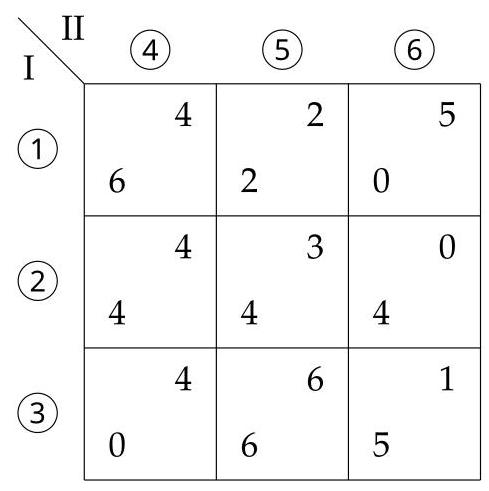
\includegraphics[width=0.4\textwidth]{images/ch09-fig20.jpg}
\end{center}
\hspace*{3em} 

(a) 找出该博弈的所有纯策略均衡。

(b) 下图展示了该博弈中参与人I和参与人II的混合策略集\(X\)和\(Y\)，但并未标明哪一个是\(X\)，哪个是\(Y\)。图中还给出了它们被划分成最优反应区域的情况，但没有任何标签，需要你加以补充。请说明哪一个三角形对应\(X\)，哪个是\(Y\)。[提示:先考虑纯最优反应。] 对于分别标记为$a, b, e$和$p, s, u$的三个顶点，指出它们各自对应的纯策略\((1,0,0), (0,1,0)\)或$(0,0,1)$，并为各个三角形标注正确的标签$\circled{1},\ldots, \circled{6}$。最后，判断该博弈是否是退化的。

\begin{center}
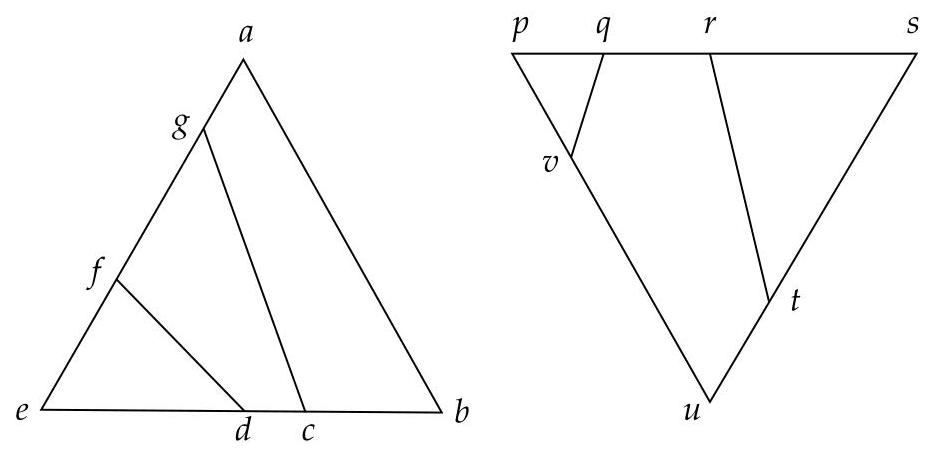
\includegraphics[width=0.7\textwidth]{images/ch09-fig21.jpg}
\end{center}
\hspace*{3em} 

(c) 根据这些标签，确定该博弈在混合策略下的所有均衡(使用标明的节点$a, b, c$, $d, e, f, g$ 和 \(p, q, r, s, t, u, v\))。

(d) 展示缺失标签1的所有莱姆基 - 豪森路径，以及它们如何连接博弈的均衡。
\end{exercise}

\begin{exercise}\label{exer:9.4}  % 9.4
考虑一个非退化的双矩阵博弈以及该博弈的任意一个纯策略均衡(假设存在)。解释为什么从$(0, 0)$开始的莱姆基 - 豪森路径总能为合适的缺失标签找到这个均衡。假设该博弈至少有两个纯均衡。解释如何使用莱姆基 - 豪森算法找到第三个(不一定是纯策略的)均衡。
\end{exercise}


\begin{exercise}\label{exer:9.5}  % 9.5
给出一个双矩阵博弈$(A, B)$的例子，其中\(A\)的每一列都有一个正元素，但式\eqref{eq:9.24}%(9.24)
中的\(Q\)不是有界多面体。
\end{exercise}


\begin{exercise}\label{exer:9.6}  % 9.6
考虑一个具有纯策略均衡的非退化双矩阵博弈。证明存在一个策略上等价的博弈，使得在这个纯均衡中，两个参与人的收益都比任何其他纯策略组合的收益严格更高。解释为什么在考虑这个等价博弈时，“囚徒困境”中的“困境”消失了。此外，给出一个例子说明需要非退化条件才能获得严格更高的收益。
\end{exercise}
